\documentclass[a4paper,12pt,twoside]{article}
\usepackage[utf8]{inputenc}
\usepackage{lmodern}
\usepackage[T1]{fontenc}
\usepackage[utf8]{inputenc}
\usepackage[icelandic]{babel}
\usepackage{geometry}
\geometry{a4paper, margin=1in}
\usepackage{fancyhdr}
\usepackage{wrapfig,graphics}
\usepackage{xcolor}     % For color support
\usepackage{hyperref}
\usepackage{csquotes,biblatex} 
\addbibresource{references.bib} 
\usepackage{float}
\usepackage{tikz}
\usetikzlibrary{automata, positioning, arrows}
% Custom blue
\definecolor{blue}{RGB}{16, 9, 159}

% Set up the color for hyperlinks
\hypersetup{
    colorlinks=true,     % Enable colored links
    linkcolor=blue,      % Color for internal links (sections, pages)
    urlcolor=blue,       % Color for URLs
    citecolor=blue,      % Color for citations
    filecolor=blue,      % Color for files
    linkbordercolor=blue % Color for boxes around links
}
\title{Lokaskýrsla: HiDef Textíll: \\ Tæknivæddar prjónavélar}
\author{Elías Lúðvíksson, Guðrún Ísafold Hilmarsdóttir\\ og Snæfríður Ebba Ásgeirsdóttir}
\date{\today}


% Set up the header for the document
\pagestyle{fancy}

% Set headers for odd and even pages
\fancyhead{}
\fancyhead[RO,LE]{
\includegraphics[width=2cm]{myndir/logo}} 

% Title in blue, centered on both odd and even pages
\fancyhead[LO,RE]{\textcolor{blue}{\leftmark}}   % `\leftmark` gets the title from \section or \chapter

% Update the footer
\fancyfoot[CO,CE]{\textcolor{blue}{\thepage}}


\begin{document}
\maketitle
\begin{abstract}
    \emph{HiDef Textíll: Tæknivæddar prjónavélar} verkefnið snýst um að sameina hefðbundna textílvinnslu og nútímatækni með nýsköpun í gömlum prjónavélum frá 10. áratugnum. Með því að snjallvæða úrelda prjónavél með netsamskiptum og frjálsum hugbúnaði verður til tól sem hentar skapandi starfi nútímans, en jafnframt stuðlar að sjálfbærni. Verkefnið er þverfaglegt og felur í sér þátttöku nemenda úr verkfræði, hagnýttri stærðfræði og fatahönnun, sem fá tækifæri til að vinna saman að þróun tækjalausna, verkefnastjórnun og frumgerðasmíði. Markmiðið var að hanna starfshæfa prjónavél sem hægt verður að kynna á ráðstefnum eins og Hönnunarmars og UTmessunni. Verkefnið stuðlar að aukinni þátttöku í STEAM menntun, þar sem listir og tækni mætast á nýstárlegan hátt, og varðveitir um leið menningararf í nútímasamhengi. Við verðum einnig á Vísindavöku Rannís 28. september nk. að kynna verkefnið fyrir almenningi, þar sem við notum vélina til að sýna samstarf háskólanna í virku sambandi við atvinnulífið.
\end{abstract}

\tableofcontents
\newpage

\section{Lýsing á verkefninu}


\begin{wrapfigure}{r}{0.5\linewidth} 
    \centering \label{img:passap}
    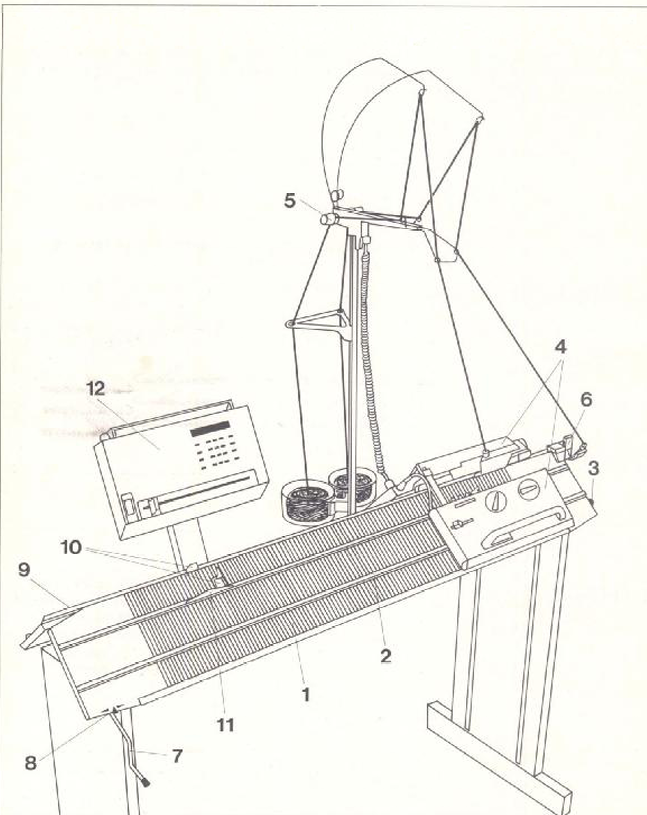
\includegraphics[width=.9\linewidth]{myndir/skema-e6000.png}
    \caption{PASSAP E6000}
\end{wrapfigure}

\subsection{Markmið}
Markmið verkefnisins \emph{HiDef Textíll: Tæknivæddar prjónavélar} er að þróa sjálfbæra og hagkvæma lausn fyrir minni hönnuði með því að uppfæra úreltar prjónavélar frá 10. áratugnum með nútímatækni, nánar tiltekið \textit{Passap E6000} (sjá mynd \ref{img:passap}). Verkefnið miðar að því að snjallvæða þessar vélar með netsamskiptum, frjálsum hugbúnaði og þróa nýtt notendaviðmót sem gerir vélarnar aðgengilegar nútímanotendum. Með því að sameina hefðbundna textílframleiðslu, sjálfbærni og nýsköpun er markmiðið að búa til tól sem hentar bæði minni hönnuðum og kennslu í STEAM greinum. Verkefnið stuðlar einnig að varðveislu menningararfs með því að færa sér\-íslensk textílmynstur úr \emph{Sjónabók} yfir í staf\-rænt, gagnvirkt form.

Við vildum einnig skrásetja ferlið gaumgæfilega til að veita nemendum innsýn í hvernig þverfaglegt samstarfsverkefni á sér stað og tengja verkefnið við kennsluskrá \emph{Háskóla Íslands} og \emph{Listaháskóla Íslands}. Með þessu er markmiðið að auðvelda nemendum skilning á því hvernig nýsköpun, tækni og listir geta unnið saman í fræðsluumhverfi og þverfaglegu samstarfi.

\subsection{Staða þekkingar}

Á alþjóðavísu hafa ýmsir hakkarar og ,,hackerspace'' unnið með gömlum prjónavélum og endurhugsað þær með nútímatækni. Dæmi um slíkt er \emph{KnitterStream} \cite{knitterstream}, sem var listagjörningur á C2-MTL ráðstefnunni í Montréal, Kanada árið 2012 þar sem gömul rafknúin prjónavél var notuð til að umbreyta tístum á Twitter í refil (sjá mynd \ref{fig:knitterstream}). KnitterStream tengdi saman gögn og prjónaframleiðslu í rauntíma og sýndi hvernig hægt væri að samþætta stafrænar upplýsingar við textílframleiðslu á skapandi hátt. Þetta verkefni var þó meira hugsað sem einnota listaverk en kennslutæki eða framleiðslulausn fyrir minni hönnuði.

\begin{figure}
    \centering
    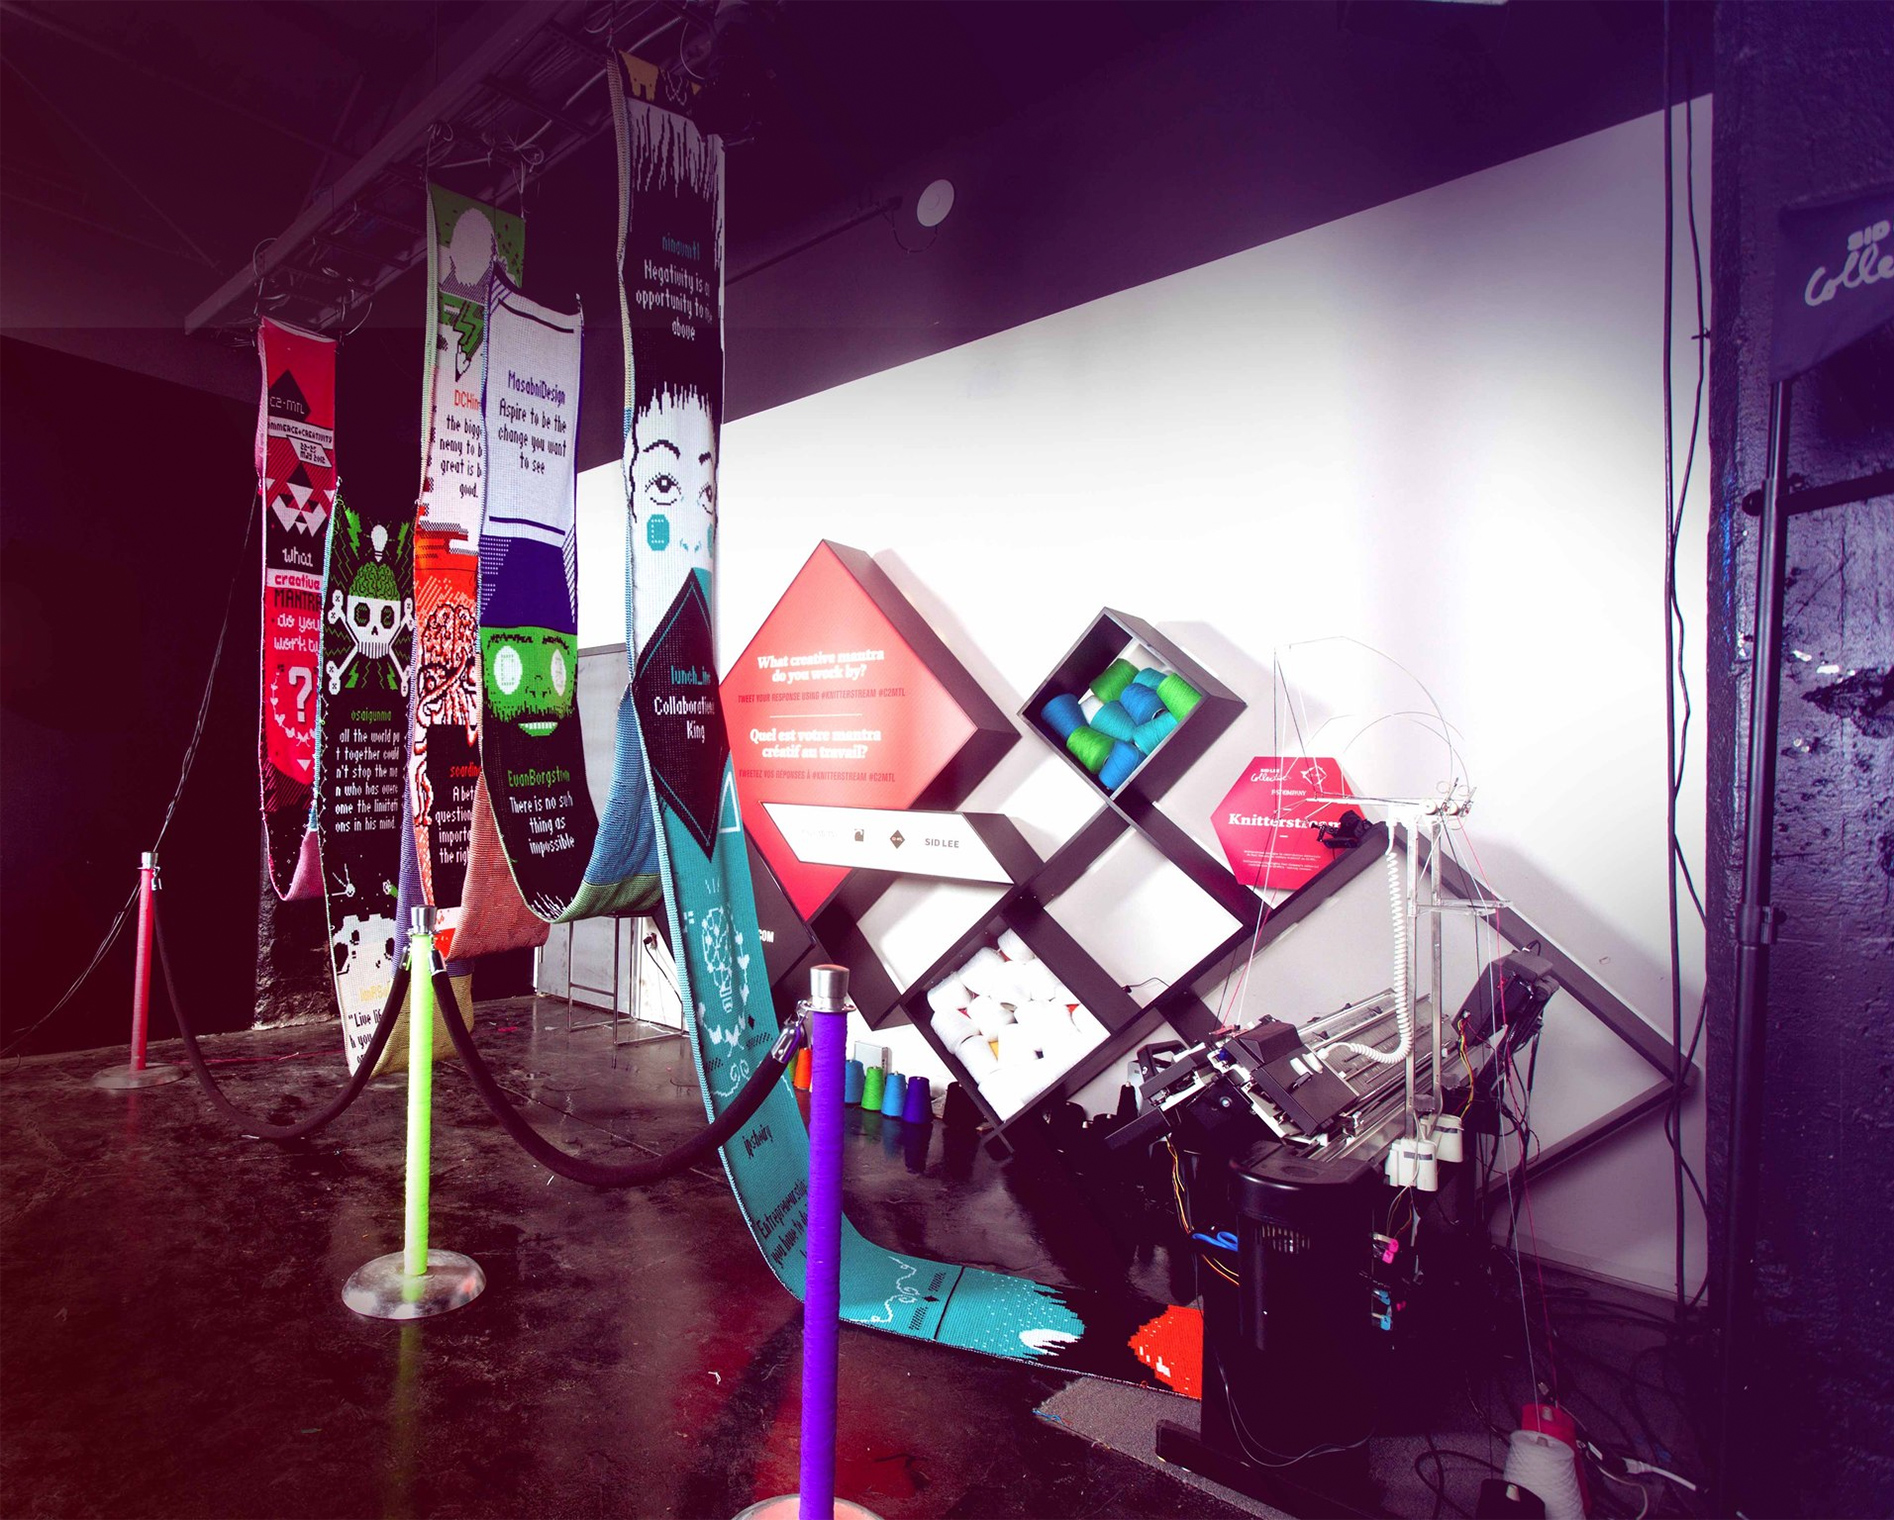
\includegraphics[height=.3\textheight]{myndir/knitterstream_24.jpeg}
    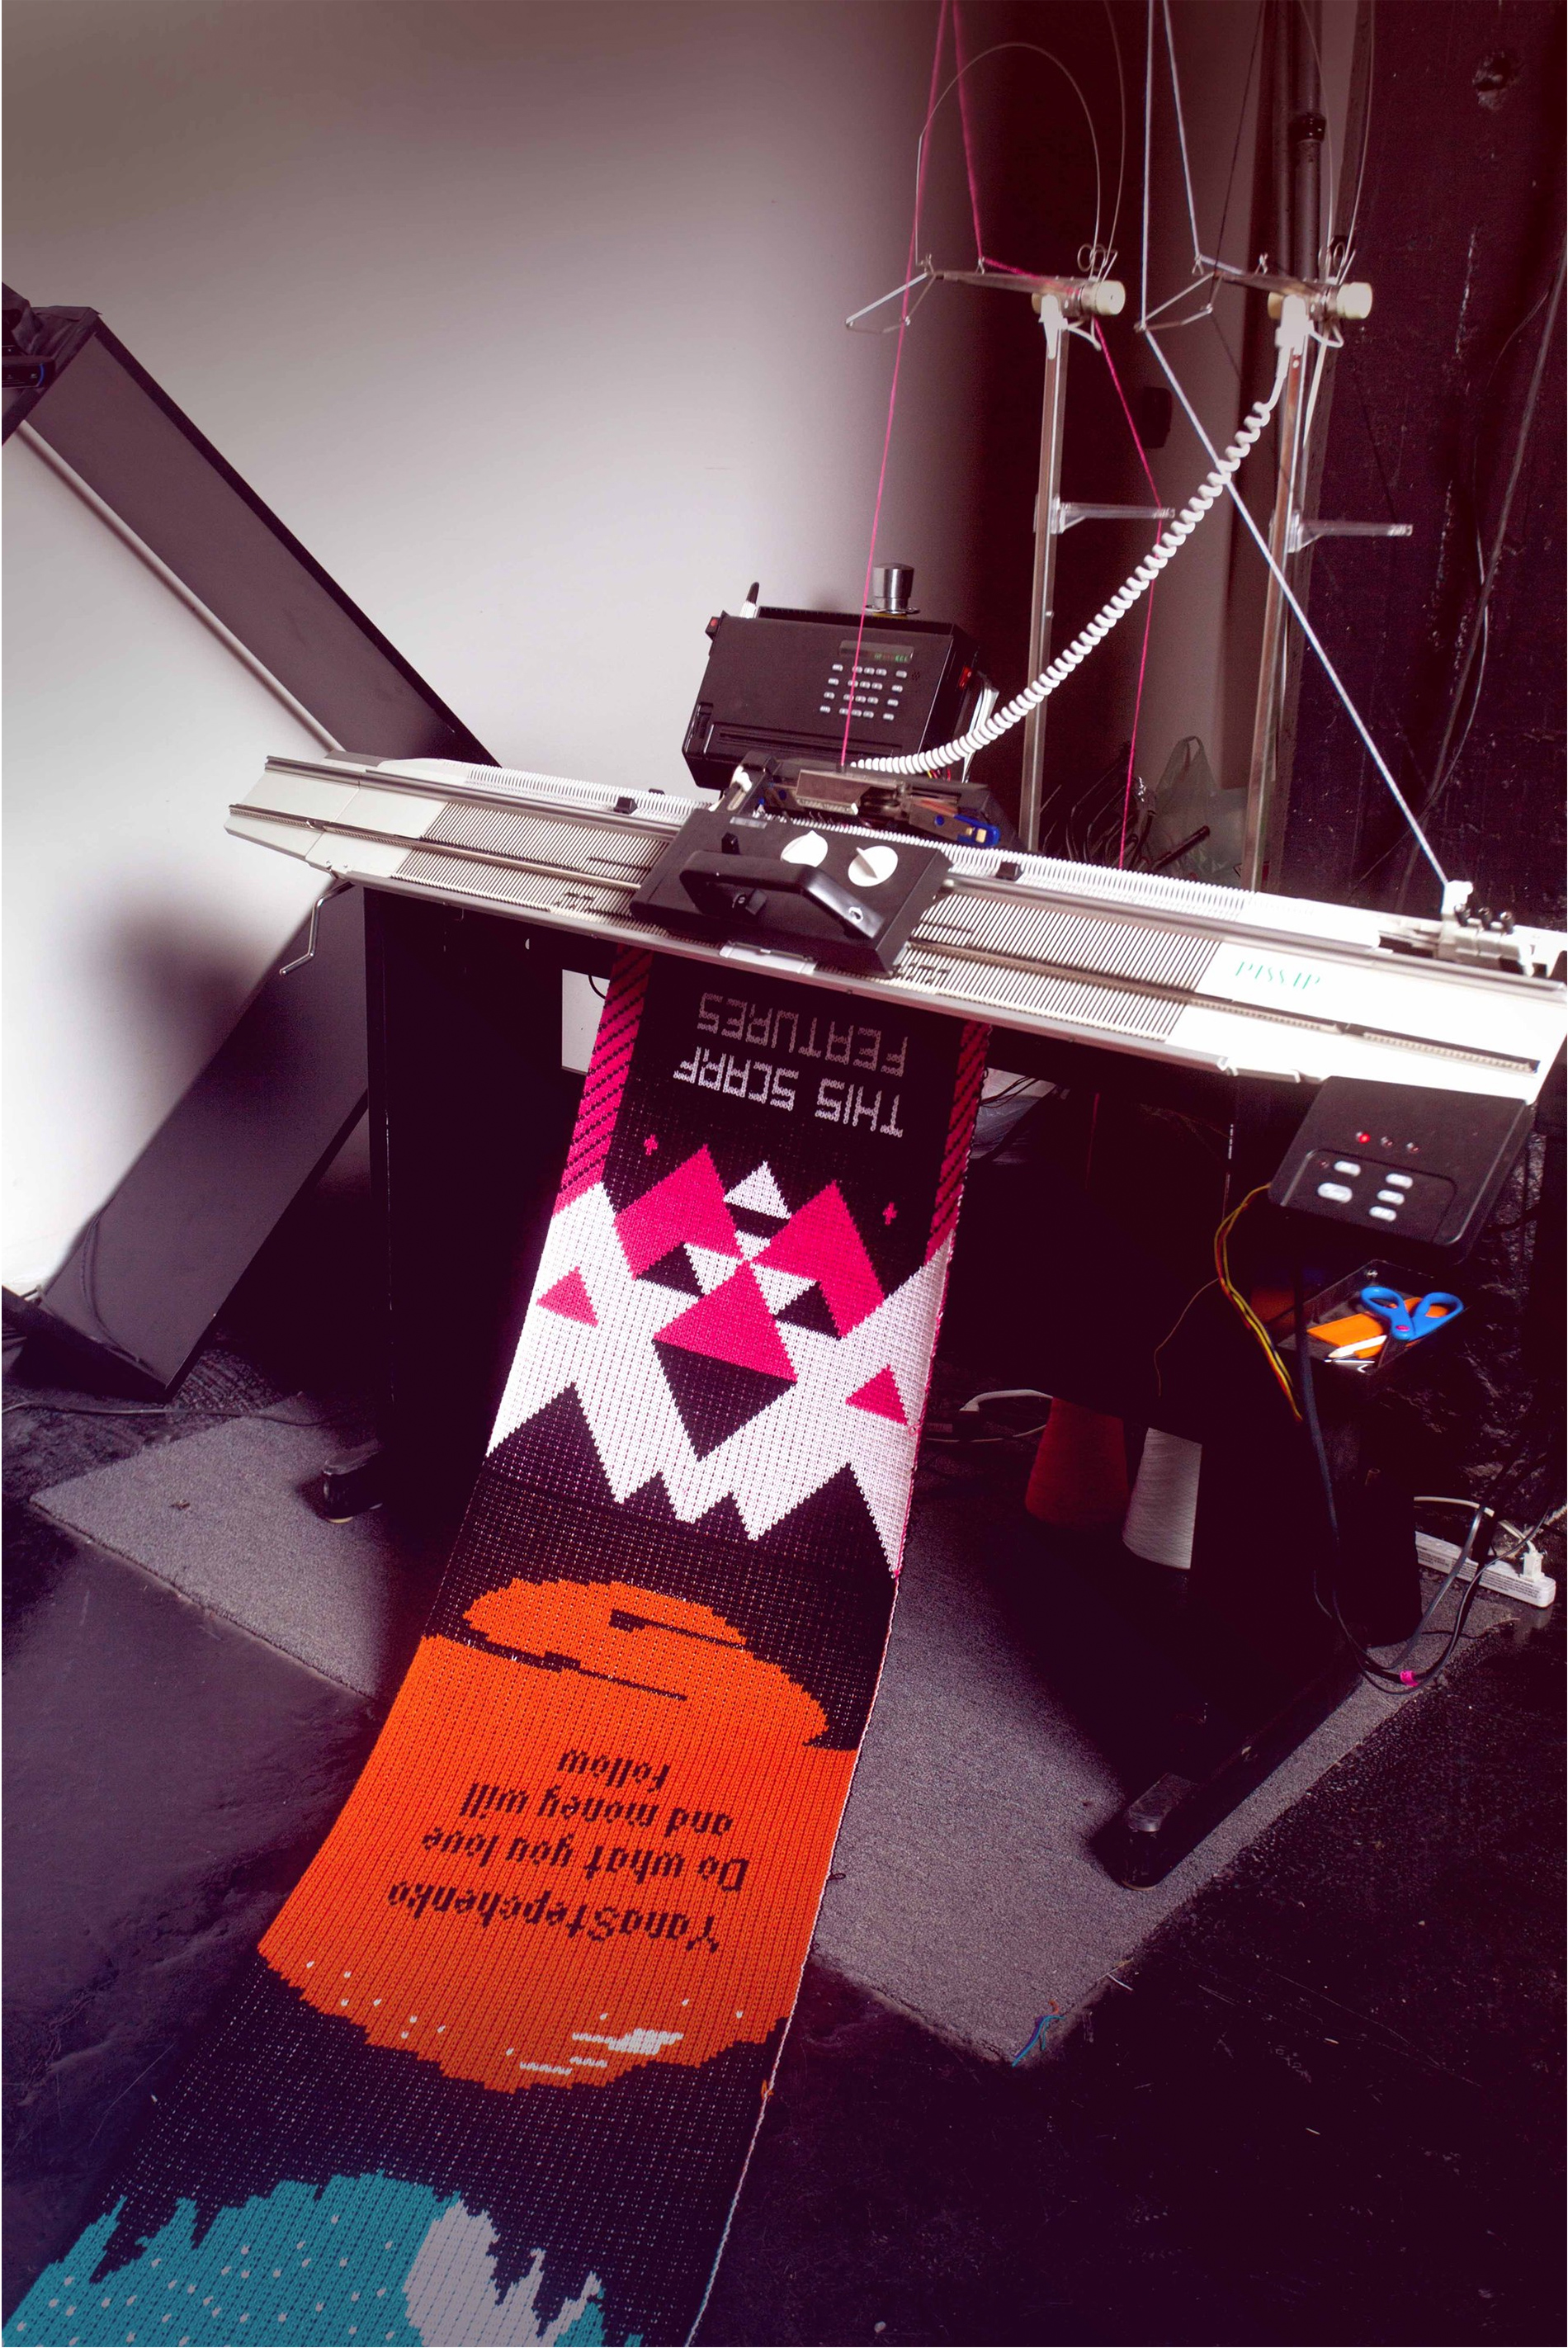
\includegraphics[height=.3\textheight]{myndir/knitterstream_25.jpg}
    \caption{Svipmyndir af KnitterStream á C2-MTL ráðstefnunni 2012}
    \label{fig:knitterstream}
\end{figure}

Einnig hafa verið unnin verkefni eins og endurbygging á \textit{Passap E6000} prjónavélinni af Backspace, Hackerspace í Bamberg, Þýskalandi \cite{bamberg}. Þar var lögð áhersla á að snjallvæða eldri prjónavél með því að koma á tengingu við nútíma hugbúnað. Irene Wolf hefur einnig þýtt og skráð hluta af þessum breytingum á ensku  \cite{irene}, en þrátt fyrir að þessi þekking sé aðgengileg almenningi, er ferlið enn frekar óljóst og þarfnaðist ítarlegri leiðbeiningar svo nýgræðingar gætu fylgt þeim eftir.

Þrátt fyrir þessi verkefni hefur skortur verið á lausnum sem einblína á kennslufræðilegt ferli eða aðgengi fyrir byrjendur sem hafa ekki mikla reynslu af vél- eða hugbúnaðargerð. Markmið okkar var að fylla þetta skarð með því að gera ferlið aðgengilegra og notendavænna fyrir þá sem vilja nota þessar vélar, en hafa ekki djúpa tæknilega þekkingu. Verkefnið einblínir á hvernig hægt er að nýta gömlu prjónavélarnar með nútíma hugbúnaði og bjóða upp á heildarlausn sem tengir saman vél- og hugbúnað á einfaldan og skýran hátt.


Okkur var einnig kært að nota séríslensk mótíf í okkar útprjóni. Við sóttum því eftir samstarfi við \emph{Heimilisiðnaðarfélagið} og \emph{Þjóðminjasafn Íslands}, sem gáfu út tímamótaverkið \emph{Íslensk Sjónabók}, sem inniheldur safn tíu handrita frá 16.-18. öld sem varðveitt hafa íslensk útsaumsmynstur \cite{Sjonabok}. Því miður er þessi bók komin úr prentun og ekki stendur til að endurprenta hana sökum kostnaðar. Markmið útgefanda var að gera mynstrin aðgengileg svo hönnuðir gætu endurnýtt okkar ríka menningararf í listsköpun sinni. Þeir tóku því vel í að við myndum veita þessum mynstrum nýtt líf og útbúa tól til að hægt væri að vinna með mynstrin á gagnvirkan hátt.


\begin{figure}
    \centering
    \begin{minipage}[b]{0.45\linewidth}
        \centering
        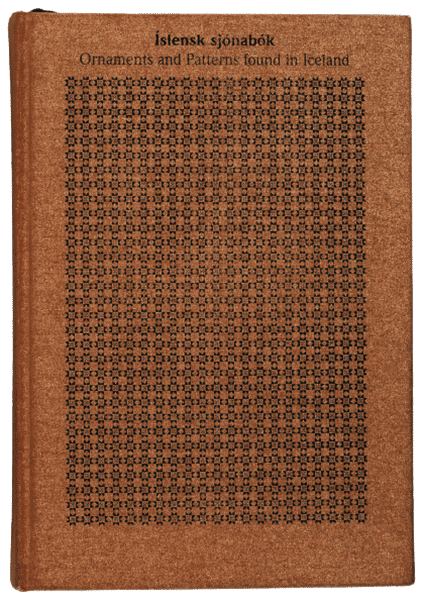
\includegraphics[width=.8\linewidth]{myndir/sjónabók.png}
        \caption{Íslensk Sjónabók}
        \label{fig:sjonabok}
    \end{minipage}
    \hspace{0.05\linewidth} % Add space between the figures
    \begin{minipage}[b]{0.45\linewidth}
        \centering
        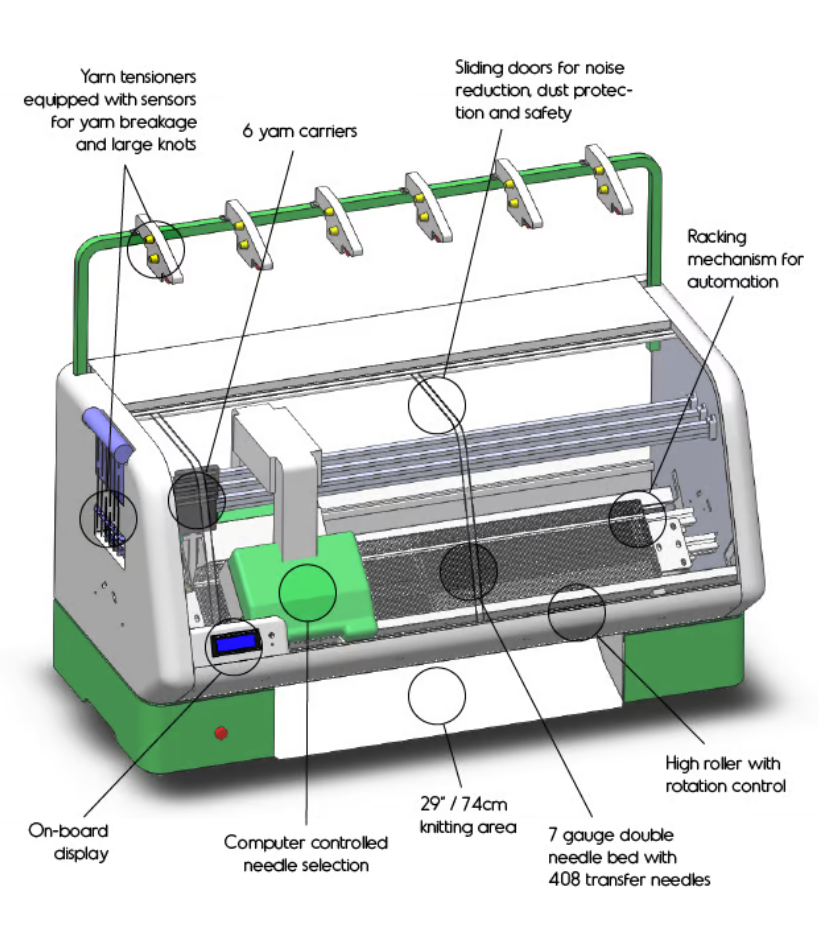
\includegraphics[width=\linewidth]{myndir/skema-kniterate.png}
        \caption{Kniterate}
        \label{fig:kniterate}
    \end{minipage}
\end{figure}



\subsubsection{Samanburður við nútíma prjónavélar}
Það eru til nútíma prjónavélar eins og \emph{Kniterate}, sem eru hannaðar sérstaklega fyrir minni hönnuði og smærri framleiðendur \cite{kniterate}. Slíkar vélar kosta þó yfir 16.000 evrur og eru tiltölulega flóknar í notkun að mati innlendra notenda. Eldri prjónavélar eins og \textit{Passap} sem við vinnum með, eru tiltölulega einfaldar í notkun, en skortir nútíma tengingar og notendavænt viðmót. Með því að snjallvæða þessar vélar og þróa hugbúnað sem gerir þær samhæfðar við nútíma framleiðsluaðferðir, getum við boðið upp á hagkvæmari og aðgengilegri lausn fyrir minni hönnuði, þar sem tæknilegt flækjustig er mun lægra.

\subsubsection{Ný viðbót við þekkingu}
Verkefnið okkar bætir við núverandi þekkingu með því að skrásetja ferlið gaumgæfilega og þróa lausn sem gerir byrjendum kleift að nýta eldri vélar með nútíma tækni. Með áherslu á kennslufræðilegt ferli og einfaldleika er markmiðið að tengja lausnina við námskrár Háskóla Íslands og Listaháskóla Íslands, svo nemendur úr ólíkum fræðasviðum geti lært af þverfaglegu samstarfi. Þetta gefur tækifæri til að búa til hönnunarferli sem tengir saman arfleifð og nýsköpun á sjálfbæran hátt, á skalanum sem hentar smærri hönnuðum og framleiðendum. Aðferðafræðin er útlistuð í kafla \ref{sec:adferdafraedi}.

\subsection{Staða verkefnis}
Verkefnið snýst um endurbætur á svissneskum prjónavélum frá 10. áratuginum, en framleiðsla þeirra hætti um aldamótin þegar \textit{Passap} fór á hausinn. Þar af leiðandi eru nýir varahlutir nánast ófáanlegir nema með því að leita að notuðum vélum og nýta hluti úr þeim sem eru enn í lagi. Þrátt fyrir að framleiðslan hafi stöðvast, eru vélarnar vel gerðar og enn í notkun af áhugafólki. Það eru virk net-samfélög sem einblína á slíkar vélar, eins og Facebook grúppur og \href{https://www.mkc.community/}{Machine Knit Community}. Auk þess eru til þónokkrar YouTube rásir sem bjóða upp á leiðbeiningar og stuðning við þessa vélar.

Forkönnun á tæknilegum og markaðslegum þáttum hefur sýnt að þörf er á hagkvæmum lausnum fyrir minni hönnuði sem vilja nýta þessar vélar, en þar sem fyrirtækið er hætt, er engin áframhaldandi þróun á þessum vélum til staðar. Verkefnið okkar miðar því að því að snjallvæða þessar vélar og tryggja að hægt sé að nýta þær á nýjan hátt með nútíma tækni og þannig auka sjálfbærni og minnka óþarfa sóun. Með því að bæta við stafrænu viðmóti og tengingu við nútíma hugbúnað, getum við komið þessum vélum í notkun sem hagkvæmari valkost fyrir smærri hönnuði og kennsluumhverfi.

\section{Nýnæmi}
\subsection{Staða markaðar}
Væntanlegur markhópur fyrir afurðina nær til minni hönnuða, listamanna, hönnunarnema og menntastofnana sem leita að hagkvæmum og sveigjanlegum lausnum til að skapa og framleiða textílvörur á sjálfbæran hátt. Markaðurinn hefur þróast í átt að sérsniðinni framleiðslu og sjálfbærni, en margar af þeim lausnum sem eru í boði, eins og \textit{Kniterate}, eru mjög dýrar og því ekki raunhæfur kostur fyrir smærri aðila. \textit{Kniterate}, sem er nútíma prjónavél hönnuð fyrir minni hönnuði, kostar um 16.000 evrur og hefur margra mánaða biðlista. Þrátt fyrir að \textit{Kniterate} bjóði upp á háþróaða tækni, er notkun hennar tæknilega flókin og því ekki aðgengileg fyrir alla.

Afurðin okkar aðgreinir sig með því að bjóða upp á hagkvæma og aðgengilega lausn sem nýtir eldri prjónavélar sem eru enn í góðu ástandi, en krefjast uppfærslu til að mæta nútímakröfum. Þar sem markmiðið er að snjallvæða þessar vélar og þróa notendavænt viðmót ásamt tengingu við nútíma hugbúnað, verður lausnin aðgengileg fyrir þá sem hafa ekki djúpa tæknilega þekkingu. Þetta skapar tækifæri fyrir smærri hönnuði og menntastofnanir til að vinna með tæki sem eru á mun lægra verði en nýrri iðnaðartæki, án þess að fórna sveigjanleika og gæðum. 

Að auki stuðlar afurðin að sjálfbærni með því að nýta eldri tæki sem annars væru ónothæf eða á leið í landfyllingu. Með því að gera þessar vélar aðgengilegar á ný, er hægt að draga úr sóun og stuðla að hringrásarhagkerfi þar sem endurnýting er í forgrunni. Lausnin er því bæði hagkvæm og umhverfisvæn og styrkir sjálfbæra þróun innan textíl- og hönnunargeirans.

\subsection{Áskoranir}
\subsubsection{Vélrænar áskoranir}
Vélrænar áskoranir fólust í því að nýta raflagnir eldri vélarinnar og bæta við spennubreytum til að tengja Arduino örtölvu við vélina. Örtölvan þarf að stilla seglastöðu prjónalássins, sem stjórnar nálarhreyfingum vélarinnar. Einnig var áskorun að tengja viðbættan mótor þannig að samskipti milli mótors, örtölvu og notenda færu rétt fram. Nákvæmni er lykilatriði til að tryggja hnökralaust prjónaferli.

\subsubsection{Hugbúnaðarlegar áskoranir}
Hugbúnaðarlegar áskoranir fólust í þróun á sjálfvirkni fyrir prjónamynstur. Upphaflega var stefnt að því að nota spunagreind til að búa til ný prjónamynstur með tækni eins og \href{https://openai.com/index/dall-e-2/}{Dall-E 2} og \href{https://www.midjourney.com/home}{Midjourney}, en það reyndist erfitt að fá áreiðanlegar niðurstöður sem fylgdu nákvæmlega okkar textaskilaboðum. Við vildum tryggja fallegt flæði milli ólíkra mynstra og skoðuðum því tækni úr tölvuleikjagerð, eins og Wave Function Collapse (WFC), sem býr til flæðandi grunnmynd eftir fyrirfram gefinni forskrift. Þessi tækni reyndist þó ekki henta okkar þörfum, og við ákváðum að þróa einfaldara módel til að bæta saman mynstrum frá ólíkum notendum með góðu flæði á milli þeirra.

\subsubsection{Prjónaáskoranir}
Prjónaáskoranir tengdust notkun innlends efniviðar. Við fengum einband á kónum frá Ístex til að nota í verkefnið, en einband er frekar gróft garn sem hentar almennt ekki vel fyrir prjónavélar. Til að mynda er ekki hægt að nota einband í \textit{Kniterate} prjónavélar án þess að það slitni í tíma og ótíma. Við prufuðum mismunandi prjónaáferðir til að finna lausn sem hentar íslensku einbandi og náðum ágætum árangri í því eftir sumarið.

Rétt spenna á garni reyndist einnig áskorun, þar sem spennugjafinn var orðinn misilla farinn fyrir ólíka garnleiðara. Þetta olli því að spennan var ójafnari, sem gat valdið vandamálum við prjónun. Einnig mynduðust stundum langir spottar á jaðri prjónastykkisins, sem tengdist spennu garnsins og því hversu langt prjónalásinn ferðast umfram það sem er prjónað. Með frekari reynslu af vélinni og tilkomu mótorvirkni, sem gerir jafnara átak á prjónið, hefur þetta batnað til muna.


\subsection{Afleidd tækifæri}
Verkefnið býður upp á fjölbreytt afleidd tækifæri, bæði fyrir hönnuði og menntastofnanir. Með því að gera eldri prjónavélar aðgengilegar og uppfæra þær með nútímatækni, eru nýir hönnuðir valdefldir til að nýta þessar vélar sem hagkvæm vinnutól í sinni sköpun. Þetta skapar aukin tækifæri fyrir sjálfstæða hönnuði og smærri framleiðendur sem vilja vinna með sjálfbærar lausnir.

Að auki geta grafískir hönnuðir nýtt munsturgerð okkar úr \textit{Sjónabók}, sem er ekki einskorðuð við prjónaskap. Mynstrin bjóða upp á margvíslega notkunarmöguleika í skapandi störfum, hvort sem það er í textílvinnu eða öðrum miðlum. Með því að færa þessi séríslensku mynstur yfir í gagnvirkt stafrænt form, opnast dyr fyrir fleiri skapandi útfærslur á þessum menningararfi.

Verkefnið býður einnig upp á möguleika á þróun nýs kennsluefnis sem getur aukið áhuga á STEAM\footnote{STEAM: Science, Technology, Engineering, Arts, and Mathematics.} námi. Með því að tengja listir og tækni á skemmtilegan og aðgengilegan hátt í kennsluumhverfi, má vekja áhuga nýrra kynslóða á þverfaglegum lausnum og nýsköpun. Þetta kennsluefni getur nýst bæði í framhaldsskólum og á háskólastigi, þar sem áhersla er lögð á samspil skapandi hugsunar, tækni og sjálfbærni.


\subsection{Hugverkastefna}
Verkefnið byggir á \textit{Free and Open Source Software} (FOSS) hugmyndafræðinni, þar sem allur hugbúnaður, tækni og aðferðir verða opnar og aðgengilegar fyrir almenning. Markmiðið er að stuðla að aukinni dreifingu og aðgengi að þeim lausnum sem þróaðar eru í verkefninu, þannig að sem flestir geti nýtt sér þær til frekari þróunar eða nýsköpunar.

Við höfum leyfi frá Heimilisiðnaðarfélaginu og Þjóðminjasafni Íslands til að dreifa mynstrum úr \textit{Sjónabók} á stafrænu formi. 

Sem rannsóknarverkefni á vegum Háskóla Íslands er allt efni og niðurstöður verkefnisins aðgengilegt í gegnum heimasíðu verkefnisins undir léni háskólans, \url{https://textill.hi.is} (vefur er ekki tilbúinn, verður opnaður fyrir nk. Hönnunarmars). Þar munu bæði kennsluefni og hugbúnaðarlausnir verða tiltækar fyrir almenning til frjálsrar notkunar og þróunar og er markmiðið að efla opið samfélag og samstarf í kringum lausnir verkefnisins.

\section{Skipulag og stjórnun}
\subsection{Stjórnun}
Verkefninu var stýrt af kennurum við Háskóla Íslands og Listaháskóla Íslands, þar sem hver kennari hafði ábyrgðarsvið sem tengist þeirra sérsviðum. Verkefnisstjóri og ábyrgðaraðili er Helga Ingimundardóttir, lektor í iðnaðarverkfræði við Háskóla Íslands. Verkefnið er hluti af rannsóknarverkefni Helgu við háskólann. Verkaskipting innan teymisins er eftirfarandi:

\subsubsection{Nemendur}
Nemendur unnu að mestu sjálfstætt, en höfðu greitt aðgengi að kennurum yfir sumarið. Hvert og eitt þeirra bar ábyrgð á útfærslu síns verkþátts:
\begin{description}
    \item[Elías Lúðvíksson] nýútskrifaður grunnnemi í vélaverkfræði við HÍ, sá um vélrænan hluta verkefnisins, þar á meðal breytingar á prjónavélinni, tengingu við mótor og samskipti við örtölvu.    
    \item[Guðrún Ísafold Hilmarsdóttir] nýútskrifaður grunnnemi í fatahönnun við Lista\-háskóla Íslands, sá um hönnunarvinnu, val á áferð og prjónaskap með íslensku einbandi.
    \item[Snæfríður Ebba Ásgeirsdóttir] grunnnemi í hagnýttri stærðfræði og tölvunarfræði við HÍ, vann að þróun spunagreindar reiknirita og að stafræna mynstur Sjónarbókar.
\end{description}

\subsubsection{Kennarar}
\begin{description}    
    \item[Hafliði Ásgeirsson] tæknimaður í frumgerðarsmiðju HÍ, veitti Elíasi leiðsögn við vélrænar breytingar og þróun frumgerðar.
    \item[Hafsteinn Einarsson] dósent í tölvunarfræði við HÍ, aðstoðaði Snæfríði við þróun spunagreindar reiknirita og tengdra hugbúnaðarlausna.    
    \item[Helga Ingimundardóttir] lektor í iðnaðarverkfræði við HÍ, er verkefnastjóri og ábyrgðar\-aðili. Hún hafði yfirumsjón með verkefninu og tryggði að það fylgdi rannsóknar\-áætlun.
    \item[Hörður Mar Tómasson] stundakennari við rafmagns- og tölvunarverkfræðideild HÍ, veitti Elíasi aðstoð við breytingar á raflögnum og tengingu við örtölvur.    
    \item[Ragna Bjarnadóttir] lektor í fatahönnun LHÍ, veitti Guðrúnu Ísafold stuðning við textíl- og hönnunarvinnu í verkefninu.
\end{description}

Stjórnskipulagið tryggir að verkefnið sé unnið á þverfaglegan hátt þar sem hver þátttakandi hefur skýra ábyrgð sem tengist þeirra sérþekkingu. Verkefnið nýtti sér hæfileika bæði kennara og nemenda til að ná fram markmiðum sínum.


\subsection{Samstarf}
Verkefnið er þverfaglegt samstarfsverkefni þar sem ólíkir aðilar, bæði innanlands og erlendis, koma að því með mismunandi sérþekkingu og aðföng. Samstarfið hefur reynst lykilþáttur í því að tryggja framgang verkefnisins og skapa tækifæri til nýsköpunar.

\subsubsection{Þjóðminjasafn Íslands og Heimilisiðnaðarfélagið}
Þjóðminjasafn Íslands og Heimilisiðnaðarfélagið veittu okkur leyfi til að vinna með mynstur úr \textit{Sjónabók} og deila þeim stafrænt með almenningi. Markmiðið er að auka útbreiðslu þessara sér\-íslensku mynstra og gera þau aðgengileg hönnuðum og almenningi til nýsköpunar og skapandi nota.

\subsubsection{Marel}
Marel veitti tæknilega ráðgjöf með breytingar á prjónavélinni. Fyrirtækið vill efla samstarf við háskóla og sá tækifæri í verkefni sem eflir hringrásarhagkerfi. Þetta samstarf stuðlar að tengingu milli iðnaðar og akademíu.

\subsubsection{Ístex}
Við fengum garn frá Ístex, sem tryggði að við værum að stuðla að hringrásarhagkerfi með því að nýta innlendan efnivið. Þetta stuðlar að sjálfbærri þróun þar sem garn úr íslenskri ull er notað í stað innfluttra efna.

\subsubsection{Textílmiðstöð Íslands}
Textílmiðstöð Íslands bauð okkur í heimsókn á Blönduós, þar sem við fengum að sjá \textit{Kniterate} vél í notkun og kynntum okkur stafrænni textílsmiðju á Íslandi. Einnig fengum við innsýn í ástand eldri prjónavéla, þar sem stofnunin hefur tekið við mörgum úreltum vélum frá dánarbúum, þar sem erfingjar vita oft ekki hvað má gera við þessar vélar.

\subsubsection{Ýr Jóhannsdóttur}
Við heimsóttum íslenskan prjónahönnuð, Ýr Jóhannsdóttur, sem deildi með okkur reynslu sinni af bæði \textit{Kniterate} og \textit{Passap} vélum. Hún hafði áður unnið á \textit{Passap} vélum áður en hún fékk loksins \textit{Kniterate} vél fyrr á árinu. Þetta samtal veitti okkur gagnlegar upplýsingar um hvernig best væri að aðlaga okkar lausnir fyrir prjónahönnuði.

\subsubsection{Owen Mace}
Við vorum einnig í reglulegu sambandi við Owen Mace, rafmagnsverkfræðing frá Ástralíu, sem hefur unnið að opnum hugbúnaði fyrir \textit{Passap} prjónavélar. Ráðgjöf hans hefur hjálpað okkur að villugreina samskipti við vélbúnaðinn. 

\subsection{Kostnaður og fjármögnun}
Verkefnið var styrkt með 9 mannmánuðum af Nýsköpunarsjóði námsmanna til að greiða sumarlaun nemenda sem tóku þátt í verkefninu. Öll önnur vinna var hluti af starfi akademískra starfsmanna, kostuð af samstarfsaðilum eða unnin í sjálfboðavinnu.

Kostnaður við breytingar á vélinni og uppsetningu á heimasíðu var greiddur af rannsóknarsjóði Háskóla Íslands sem hluti af rannsóknarverkefni Helgu Ingimundardóttur, \textit{HiDef Textíll: Bestun á textílferlum með gervigreind}. Ístex styrki okkur með íslensku einbandi.

\section{Verðmæti}
\subsection{Viðskiptaleg markmið}
Verkefnið miðar að því að stuðla að opnu aðgengi og valdeflingu nýrra hönnuða með því að bjóða upp á opnar lausnir fyrir \textit{Passap} prjónavélar og útbreiðslu mynstra úr \textit{Sjónabók}. Við viljum gera \textit{Passap} prjónavélar að aðgengilegum vinnutækjum fyrir hönnuði sem geta nýtt þær í sköpun sína án þess að þurfa að leggja í of háan startkostnað. Einnig viljum við styðja við útbreiðslu mynstra úr \textit{Sjónabók} með því að gera þau aðgengileg á stafrænu formi fyrir almenning.

Varan sjálf er í raun kennsluefni og þekkingin sem hefur safnast í verkefninu, sem sýnir hvernig hægt er að vinna með þverfaglegt samstarf innan háskólasamfélagsins og innlend fyrirtæki. Verkefnið leggur áherslu á að skapa verðmæti með því að stuðla að fræðslu og hagnýtum lausnum fyrir hönnuði og menntastofnanir, frekar en að stefna að hefðbundnum markaðshlutdeild og veltu.

\subsection{Leið á markað}
Til að auka útbreiðslu og kynna verkefnið fyrir breiðum hópi, höfum við nú þegar kynnt það fyrir \href{https://www.mkc.community/about-us}{Machine Knit Community}, alþjóðlegum hópi notenda prjónavéla, sem hefur leitt til áhuga og beiðna um frekari upplýsingar. Við höldum einnig úti Instagram síðu, \href{https://www.instagram.com/hideftextiles/}{@hideftextiles}, þar sem við deilum uppfærslum um verkefnið með fylgjendum okkar, bæði innlendum og erlendum.

Áætlunin er að kynna verkefnið á innlendum ráðstefnum og viðburðum, svo sem á Vísindavöku Rannís (28. september nk.) og á Hönnunarmars 2025. Auk þess höfum við fengið vilyrði frá Hönnunarsafni Íslands um að halda opna vinnustofu fyrir sumarið 2025, þar sem almenningur getur kynnt sér verkefnið og möguleikana sem það býður upp á.

\subsection{Almenn verðmætasköpun}
Niðurstöður verkefnisins geta stuðlað að aukinni verðmætasköpun á Íslandi með því að stuðla að sjálfbærni, varðveislu menningararfs og valdeflingu minni hönnuða. Með því að bjóða upp á opnar lausnir fyrir snjallvæðingu eldri prjónavéla eins og \textit{Passap}, skapast tækifæri fyrir smærri hönnuði til að nýta þessar vélar á hagkvæman hátt í sinni framleiðslu. Þetta gerir nýsköpun innan textíliðnaðarins aðgengilegri og lækkar þröskuldinn fyrir þá sem vilja þróa sín eigin vöru á hagkvæman hátt.

Verkefnið styður við sjálfbæra þróun með því að leggja áherslu á endurnýtingu eldri véla og innlends efniviðar eins og íslenskrar ullar. Í stað þess að henda úreltri tækni, snýst verkefnið um að snjallvæða þessi tæki og koma þeim aftur í notkun. Þetta stuðlar að hringrásarhagkerfi þar sem verðmæti er skapað úr því sem annars gæti farið til spillis.

Að auki bætir verkefnið við íslenskan menningararf með því að gera mynstur úr \textit{Sjónabók} aðgengileg í stafrænu formi. Þessi sér\-íslensku mynstur geta nýst í fjölbreyttum skapandi verkefnum, bæði innanlands og utan. Með því að opna fyrir notkun þessara mynstra styður verkefnið við varðveislu íslenskrar arfleifðar og gerir hana að hluta af samtímahönnun.

Verkefnið getur einnig haft jákvæð áhrif á menntun og nýsköpun með því að tengja listir, tækni og menningararf. Með því að þróa kennsluefni sem tengir saman STEAM greinar, stuðlum við að aukinni vitund og áhuga á þverfaglegri nýsköpun. Þetta getur eflt samstarf innan menntastofnana og skapað tækifæri fyrir nýsköpun sem byggir á bæði tækni og sköpunargáfu.

Þannig er verðmætasköpunin sem verkefnið stuðlar að ekki bundin við tekjur af einstaka afurðum, heldur við fjölþættan stuðning við sjálfbærni, nýsköpun, menntun og varðveislu íslenskrar menningararfleifðar.

\section{Framkvæmd verkefnisins}
Hér er farið yfir hvernig verkefnið var framkvæmt, með áherslu á þrepaskiptingu, helstu áfanga og tímalínu. Verkefnið var skipt í nokkur lykilþrep, þar sem hverjum áfanga var stýrt af ákveðnum ábyrgðaraðilum. Prjónavélin var til húsa í vélaskála VR-III (sjá mynd \ref{fig:workshop}) við Hjarðarhaga 2 í Reykjavík. Nemendur höfðu einnig aðgang að Sprotamýri, frumkvöðlasetri HÍ í Grósku.

\begin{figure}
    \centering
    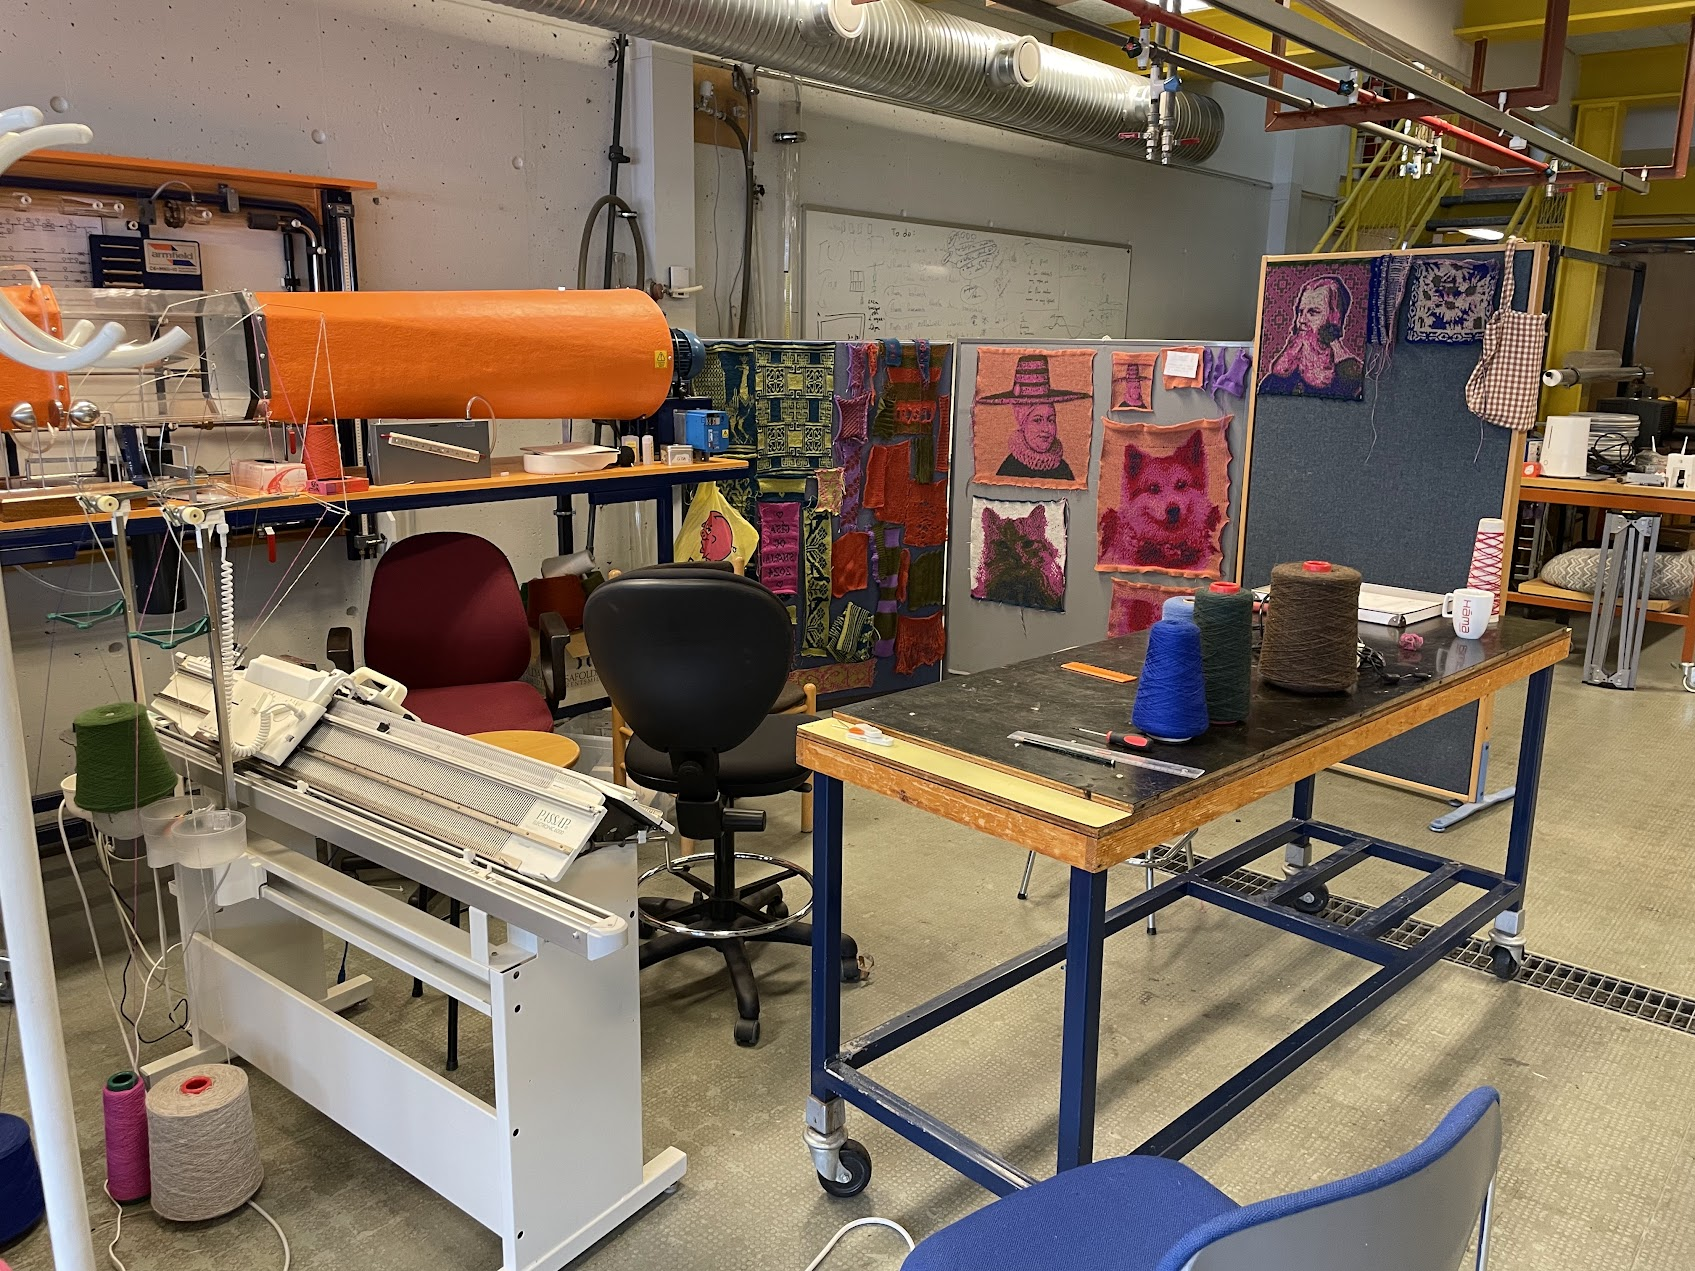
\includegraphics[width=0.9\linewidth]{myndir/workshop.jpg}
    \caption{Verkefnið var unnið í vélaskála VR-III.}
    \label{fig:workshop}
\end{figure}

\subsection{Tímalína verkefnisins}
\subsubsection{Daglegt stand-up}
Unnið var í verkefninu frá maí til miðjan ágúst þegar kennsla hófst á ný. Til að halda utan um tímalínu verkefnisins var notað \href{https://geekbot.com/}{GeekBot} á \textit{Teams} svæði þátttakenda verkefnisins. Á hverjum virkum degi fengu nemendur fjórar spurningar til að svara, sem voru:
\begin{enumerate}
    \item Slembin spurning til að nemendur kynnast hvort öðru -- svokallaðir ,,icebreakers''
    \item Hvað hefur þú gert síðan síðast? en kerfið gaf þeim upp síðasta svar sem þau gáfu við lið 3.
    \item Hvað ætlar þú að gera í dag?
    \item Þarftu hjálp við eitthvað?
\end{enumerate}
Þannig gátu kennarar fylgst með framgangi nemenda yfir sumarleyfistímabil, og viðeigandi sérfræðingur komið inn eftir þörfum. Mynd \ref{fig:geekbot} sýnir stand-up svörun yfir sumarið, en stundum voru fundir gerðir í persónu í staðinn. 

Kosturinn við að gera þetta á þennan máta er að við höfum eftir sumarið mælanlegt tímaplan fyrir hvað hver liður tók, og hvað voru helstu flöskuhálsar. Hlutir sem eiga til með að gleymast ef ekki er skrifað strax niður.

\begin{figure}
    \centering
    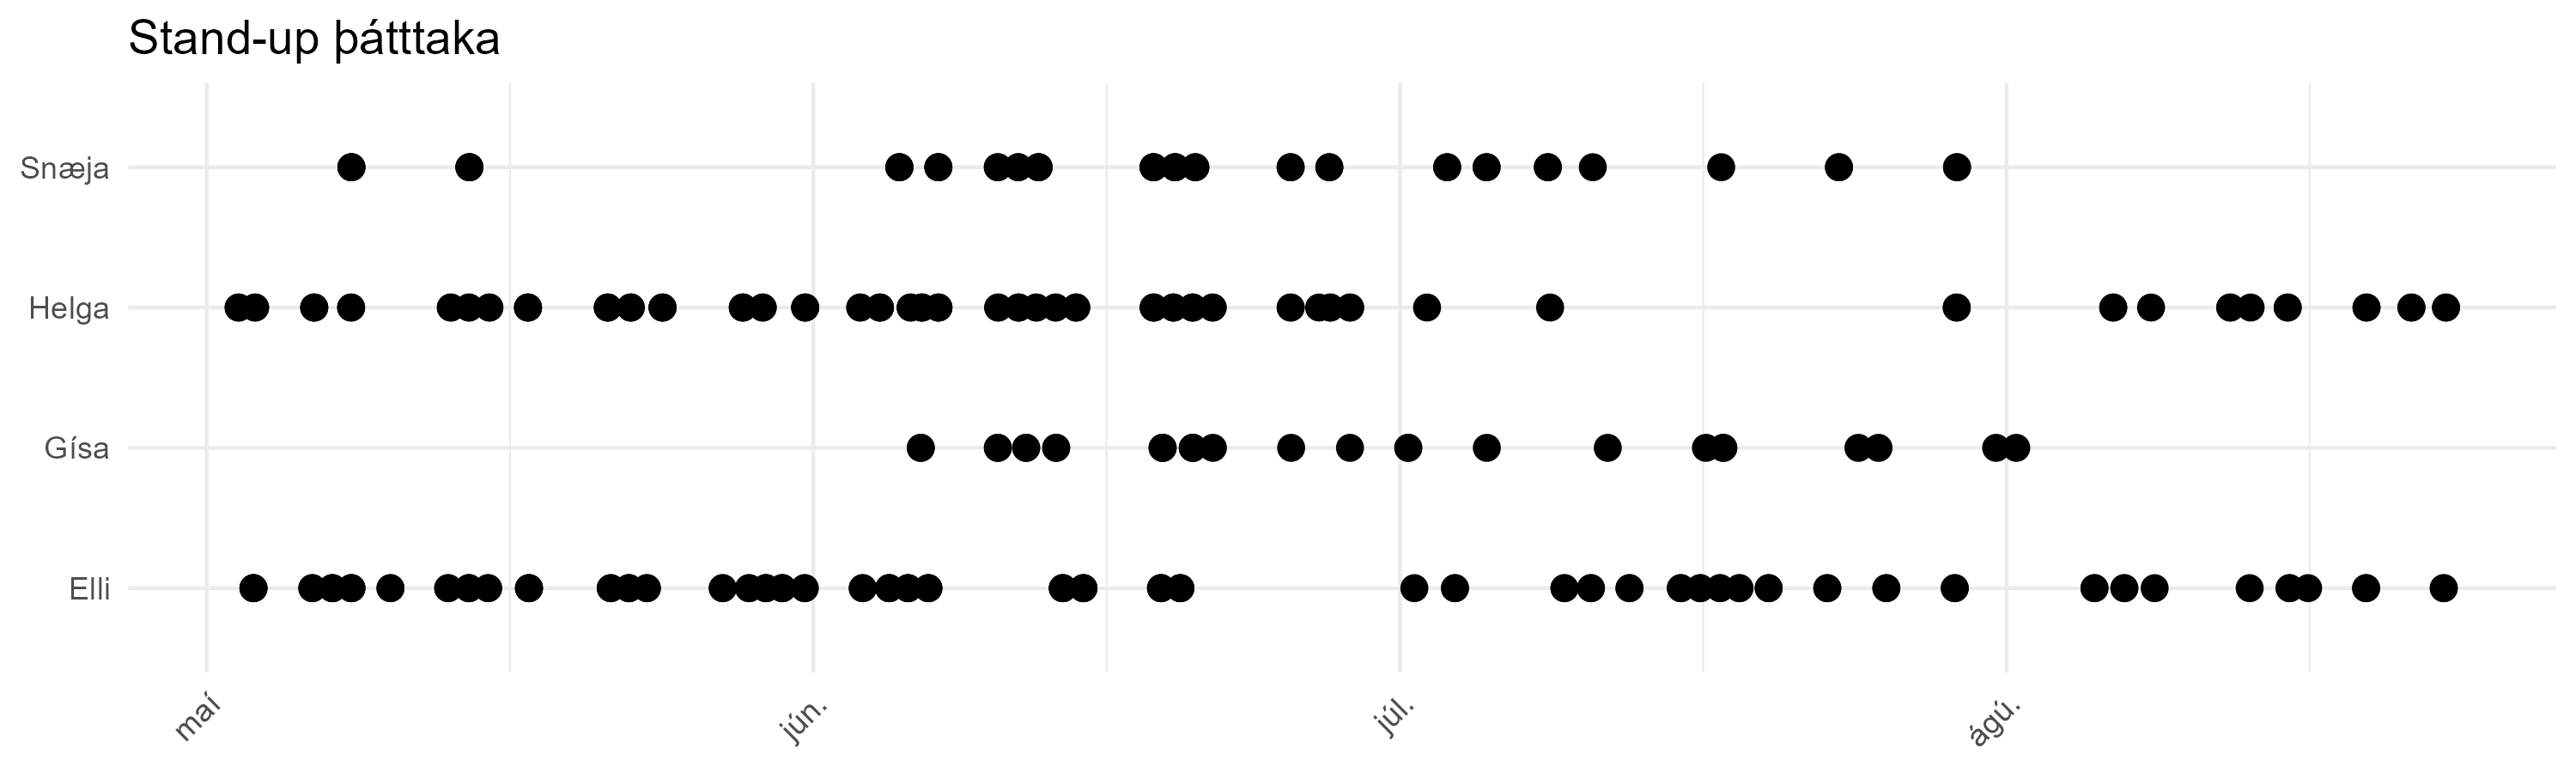
\includegraphics[width=0.8\linewidth]{myndir/standup.png}
    \caption{Þátttaka í tímaóháðu stand-up með \textit{GeekBot}}
    \label{fig:geekbot}
\end{figure}

\subsubsection{Mánaðarlegt yfirlit}
\begin{description}
    \item[Maí 2024:] Forkönnun og undirbúningur.  
    \begin{description}
        \item[Elías] TODO
        \item[Guðrún Ísafold og Snæfríður] Þrif og undirbúningur á vél.
    \end{description}
    \item[Júní 2024:] Sambærileg verkefni voru skoðuð til að fá hugmyndir, vélbúnaður var prófaður og byrjað var að skrifa kóða til að senda mynstur til vélarinnar.
    \begin{description}
        \item[Elías] TODO
        \item[Guðrún Ísafold] TODO
        \item[Snæfríður] Sambærileg verkefni skoðuð fyrir hugmyndir. Lærði á vélina og hvernig hún prjónar, skiptir um liti, prjónar mynstur o.fl. Prufugerðir og tengst vélinni í fyrsta skipti. Byrjað að skrifa kóða sem vinnur mynstur til að senda á vélina. Heimsóknir í heimilisiðnaðarfélagið, prjónaverksmiðjuna Kidka, textílsetrið á blönduósi og vinnustofuna hjá Ýrúrarí.
    \end{description}
    \item[Júlí 2024:]  Mynstur voru færð yfir á tölvutækt form, kóði skrifaður til að vinna með þau á ýmsan hátt, og prufugerðir á vélinni voru framkvæmdar þrátt fyrir tæknileg vandamál.
    \begin{description}
        \item[Elías] TODO
        \item[Guðrún Ísafold] TODO
        \item[Snæfríður] Sjónabókarmunstrum komið yfir á tölvutækt form. Kóði skrifaður sem vinnur með munstrin á ýmsan máta, bæta við borða, bæta við bakgrunni á myndir og skrifa texta. Kóði sem breytir myndum (\texttt{jpg} og \texttt{png}) í prjónamynstur skrifaður. Haldið áfram með prufugerðir sem var ansi tímafrekt þar sem mótorinn var ekki kominn í gang, lentum í ýmsum vandræðum með vélina og fundum út úr því hvernig er hægt að prjóna með 4 litum. Fórum í heimsókn á Þjóðminjasafnið fyrir innblástur og til að skoða hvernig íslensku munstrin voru notuð og tókum fund með Lilju starfsmanni Þjóðminjasafnsins sem upplýsti okkur meira um sjónabækurnar.
    \end{description}
    \item[Ágúst 2024:] Fleiri prufugerðir framkvæmdar, kóði fínpússaður, búinn til samskiptastaðall til að eiga við vélina, þar sem mynstur eru send á miðlægan gagnagrunn og lesin þaðan.
    \begin{description}
        \item[Elías] TODO 
        \item[Guðrún Ísafold] TODO
       \item[Snæfríður] Enn fleiri prufur og kóði fínpússaður. Mynsturgerð með Wave function collapse reikniritinu útfærð og byrjað á að þróa aðferð til að lita sjónabókarmunstrin sjálfvirkt. Fór á námskeið hjá Hafliða um þrívíddarprentun.
    \end{description}
    \item[September 2024:] Kynning verkefnisins. Fyrstu kynningar á verkefninu fóru fram á Vísindavöku Rannís, þar sem verkefnið var kynnt almenningi. 
    \begin{description}
        \item[Allir] Skýrslugerð og kynning á Vísindavöku.
    \end{description}
\end{description}

\subsection{Helstu áfangar}
\begin{description}
    \item [Stýring á seglum] Við tengdum \textit{Arduino} örtölvu við \textit{Passap E6000} þannig að hægt var að senda skilaboð á vélina um hvaða hjálpanálar ættu að fara í virka eða óvirka stöðu. 
    \item [Tenging við mótor] Við tengdum \textit{Arduino} örtölvu við \textit{Passap E6000} þannig að hægt var að ferja sleðann sjálfvirkt fram og aftur á prjónaborðinu með mótor. 
    \item [Samskiptastaðall] Við hönnuðum samskiptastaðal fyrir prjónavélina, þannig að mynstur frá notenda eru sett á miðlægan gagnagrunn, \textit{Arduino} örtölvan les þaðan hvaða mynstur eru á bið og stýrir seglum og mótor eftir þeirri forskrift. 
    \item [Stafræn Sjónabók] Mynstur úr \textit{Sjónabók} voru til á tölvutæku formi sem \texttt{.eps} myndir sem við myndgreindum svo hægt væri að þýða það yfir í handhægara textaform svo hægt væri að vinna með það áfram. 
    \item [Einfalt hönnunarviðmót] til að vinna með grunnmynstur \textit{Sjónarbókar}, breyta litavali og eiga við einstaka pixla.
    \item [Prjónaprufur] Tilraunir með íslenskt einband og mynstur voru lykilatriði til að tryggja að vélin gæti prjónað á áreiðanlegan hátt með innlendum efnivið.
    \item [Kynning verkefnisins] Verkefnið verður kynnt fyrir breiðum hópi á Vísindavöku Rannís í lok september 2024 og munu frekari kynningar fara fram á Hönnunarmars 2025 og á vinnustofu í Hönnunarsafni Íslands næsta sumar.
\end{description}

\section{Aðferðafræði}\label{sec:adferdafraedi}
\subsection{Breytingar á vélbúnaði}
Vélbúnaður prjónavélarinn er í grófum dráttum:  nálarbeðið, sleðinn/lásinn, litaskiptirinn og mótorinn.

\begin{figure}[H] % <- ekki taka út H þá fara myndirnar á flakk.
    \centering
    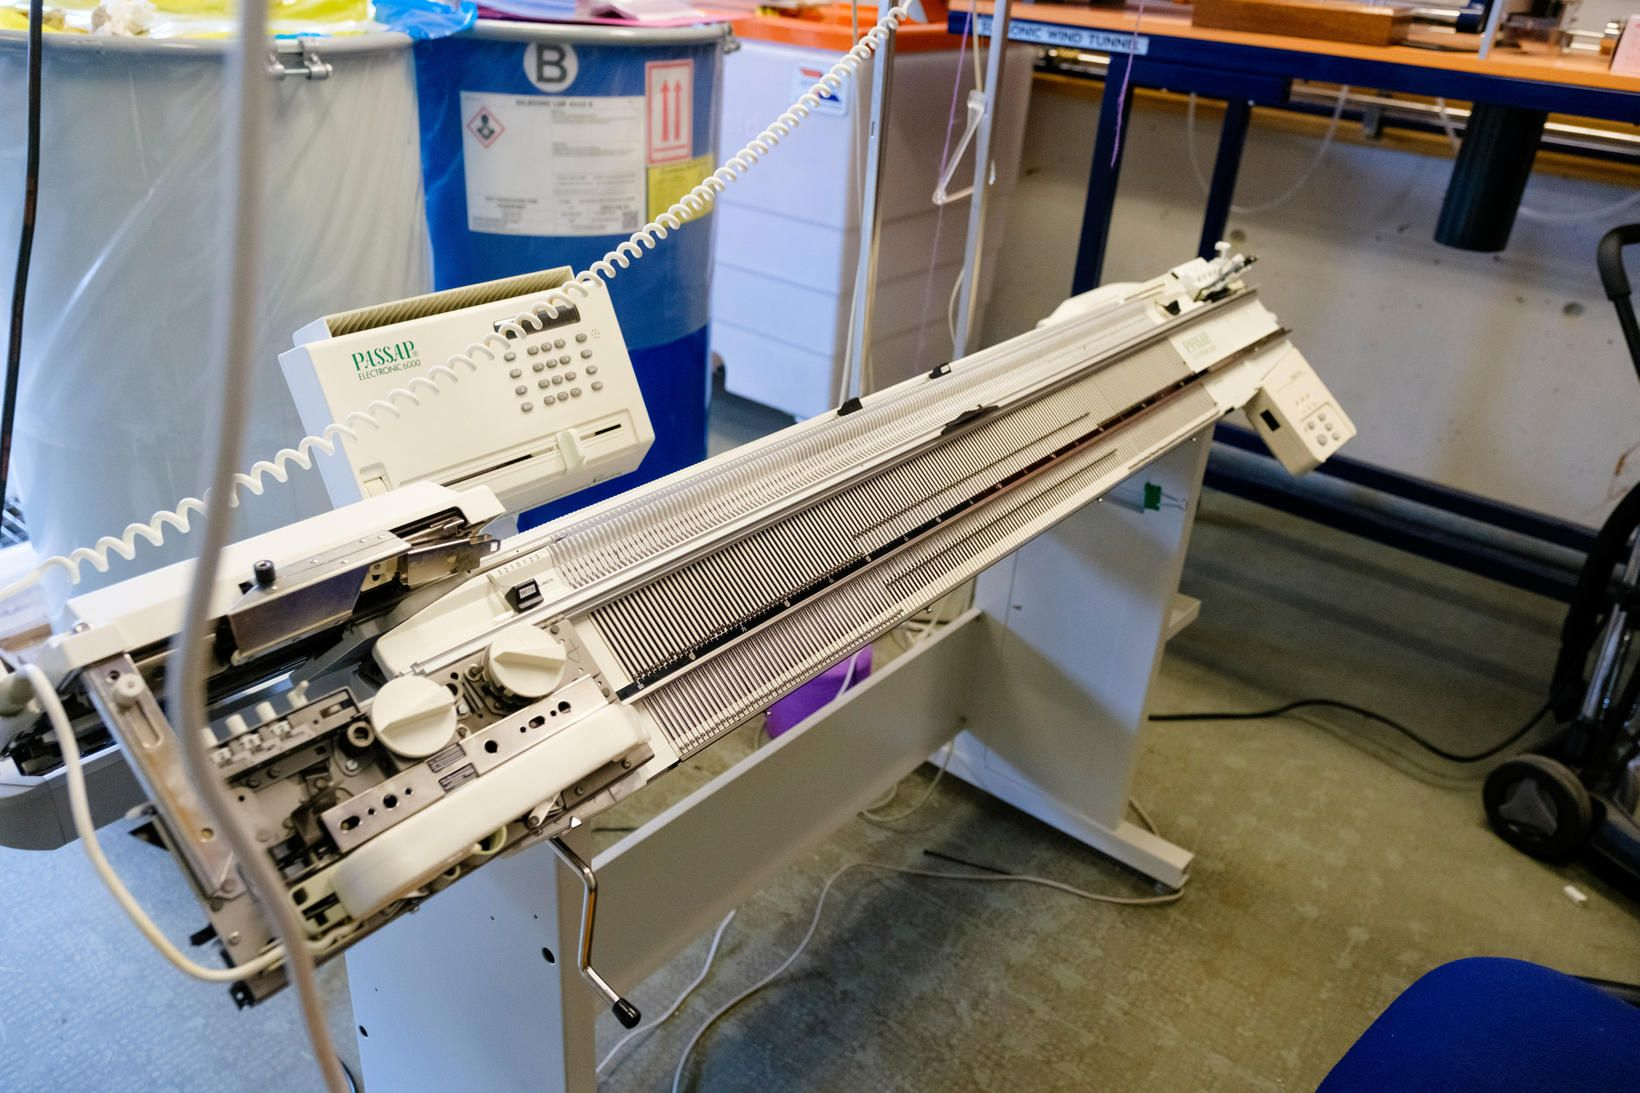
\includegraphics[width=0.5\linewidth]{myndir/elli/e6000.jpg}
    \caption{\textit{Passap E6000} prjónavél - \textit{mbl.is/Kristinn Magnússon}}
    \label{fig:e6000}
\end{figure}
\begin{enumerate}
    \item \textbf{Nálarbeðið inniheldur}
\begin{itemize}
    \item Braut sem sleðinn rennur eftir
    \item Nálastillara (e. pushers) sem eru undir nálunum í nálabeðinu og ýta nálunum í prjónastöðu. \\
    Þeir eru notaðir til að slökkva og kveikja á nálum fyrir hverja umferð, þ.e.a.s. setja nálar í óvirka eða virka stöðu.
    \item Nálarnar sem prjóna lykkjurnar ef þær eru í réttri stöðu þegar sleðinn fer yfir þær.
\end{itemize}
    \item \textbf{Sleðinn/lásinn samanstendur af}
    \begin{itemize}
        \item Tvo ljósaskynjara sem eru notaðir til að staðsetja sleðann á nálabeðinu.
        \item Tvo segla sem setja stöðu nálastillaranna fyrir næstu umferð.
        \item Braut sem fer með nálar í eftir tveimur mögulegum leiðum: 
        i) upp og prjónar lykkju í garninu eða ii) niður og prjónar ekki lykkju.
    \end{itemize}
    \item \textbf{Litaskiptirinn}
    \begin{itemize}
        \item Geymir garn.
        \item Er með einskonar takka sem sleðinn virkjar þegar hann fer yfir og skilar garni. Þá er nýtt garn sett í virka stöðu og það tekið upp á bakaleiðinni.
    \end{itemize}
    \item \textbf{Mótorinn} 
    \begin{itemize}
        \item Snýr belti sem hefur festingu fyrir sleðann.
        \item Festingin er með segul.
        \item Það eru þrír skynjarar á umgjörðinni sem inniheldur beltið sem skynja segulinn.
    \end{itemize}
\end{enumerate}
Hægt er að skipta vélbúnaðinum upp í tvö stýrikerfi. Annars vegar stýringin á mótornum sem færir sleða lásinn frá vinstri til hægri yfir nálabeðið. Hinsvegar stýringin á seglunum sem færa nálastillara á nálabeðinu upp og niður. Fyrir hvern nálastillir sem er stillt upp er lykkja prjónuð með garni fyrir þá nál í næstu umferð.
\subsubsection{Stýring nálarbeðs}
Upprunalega \textit{Passap E6000} vélin er með stjórnborð (svokölluð \textit{Form} tölva) sem er tengd með DIN-6 snúru við sleðann sem er læstur á nálabeðinu. Sleðinn er
með rafrás sem hefur ljósskynjara sem skynja göt á brautinni sem sleðinn rennur eftir. Götin eru \textit{2mm} breið og það eru \textit{3mm} á milli gata. Hver nál er \textit{5mm}. 

Mynd \ref{fig:original-pusher-control} er kerfismynd af kerfinu sem stýrir nálastillurunum á nálabeðinu. Upprunalega stjórnborðinu var skipt út fyrir \textit{Arduino} með \textit{12v} spennubreyti sem er beintengdur við sleðann.

\begin{figure}[H] % <- ekki taka út H þá fara myndirnar á flakk.
    \centering
\begin{tikzpicture}[auto, node distance=2cm, >=latex']

    % Define nodes
    \node [rectangle, draw, align=center] (sensor) {Ljósskynjari};
    \node [align=center, left=2cm of sensor] (light) {braut};
    \node [rectangle, draw, align=center, right=4cm of sensor] (sled) {Sleði/Lás};
    \node [rectangle, draw, align=center, above=3cm of sled] (console) {Stjórnborð};
    \node [rectangle, draw, align=center, below=3cm of sled] (magnets) {Seglar};
    \node [align=center, below=1.5cm of magnets] (needle) {Nálastillir};
    \node [align=center, above=0.5cm of console] (power) {Spennubreytir};
    % \node {align=center, above=1cm of arduino} (power) {spe}
\draw[->] (light) edge[dotted, above] node{ljós} (sensor)
          (light) edge[dotted, below] node{skuggi} (sensor)
          (sensor) edge[above] node{hár straumur} (sled)
          (sensor) edge[below] node{lágur straumur} (sled)
          (sled) edge[->, dashed, right] node[rotate=-90, above] {hár straumur} (magnets)
          (sled) edge[->, dashed, left] node[rotate=-90, below] {lágur straumur} (magnets)
          (console) edge[dashed, left] node[rotate=90, below] {} (sled)
          (power) edge[dashed, above] node[above] {} (console)

          % Dashed line from console to sled coming out from the right side of the console with arrow only at the end
          (console.east) edge[bend left] node[rotate=-90, above] {hár straumur} (sled.east)
          (console.east) edge[bend left] node[align=center, rotate=-90, below] {lágur\\ straumur} (sled.east)
                    (sled.west) edge[bend left] node[rotate=90, above] {hár straumur} (console.west)
          (sled.west) edge[bend left] node[align=center, rotate=90, below] {lágur\\ straumur} (console.west)
          (magnets) edge[dotted] node[rotate=-90, above] {niður} (needle)
                    (magnets) edge[dotted] node[rotate=-90, below] {upp} (needle)
          ;
        \node[draw, rectangle, anchor=north west] at (1, -4.5) {
        \begin{tikzpicture}[x=1cm, y=0.8cm]
            \draw[thick] (0,0) -- (1,0) node[right] {5V};
            \draw[thick, dashed] (0,-0.5) -- (1,-0.5) node[right] {15V};
        \end{tikzpicture}
    };\end{tikzpicture}
    \caption{Stýring sem stillir nálar prjónavélarinar}
    \label{fig:original-pusher-control}
\end{figure}

\begin{figure}[H] % <- ekki taka út H þá fara myndirnar á flakk.
    \centering
    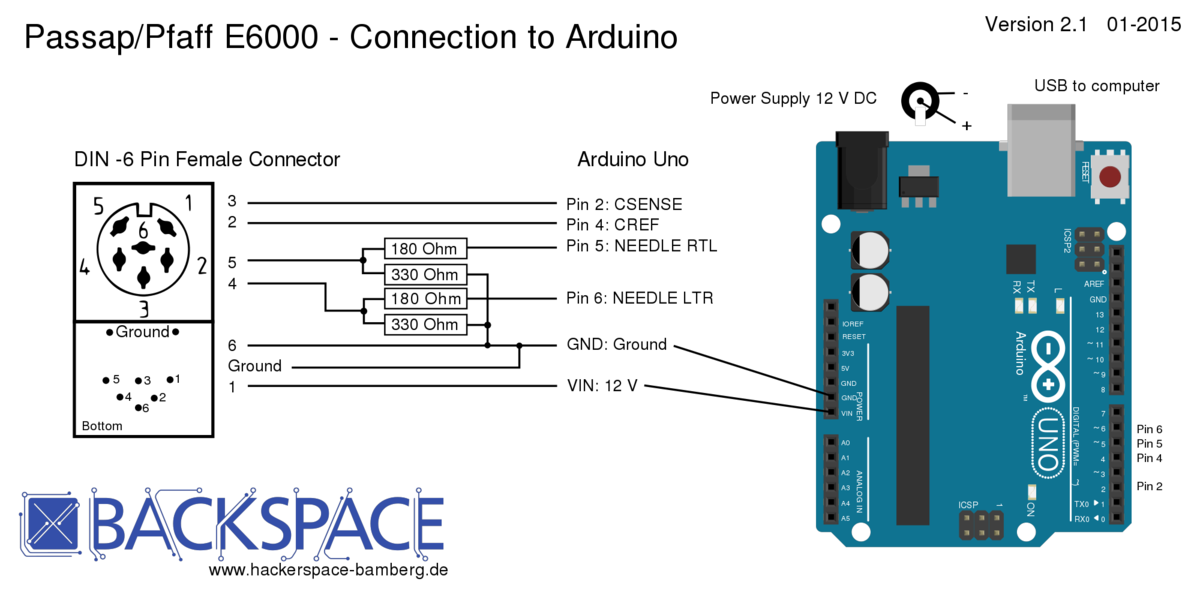
\includegraphics[width=0.75\linewidth]{myndir/bambergDIN6.png}
    \caption{Teikningar fyrir tengingu í gegnum DIN tengið voru fengnar af vefsíðu Bamberg \cite{bamberg}. }
    \label{fig:bambergDIN6}
\end{figure}
Pinnar 2 og 4 taka við straum frá ljósaskynjurum sleðans. Pinnar 5 og 6 stýra stöðu seglana tveggja. 
Það er einn segull fyrir hvorra áttina. Sleðinn stillir munstur fyrir næstu umferð á meðan hann fer yfir nálarbeðið og prjónar  munstrið sem er nú þegar á nálarbeðinu. Til að snúa við seglunum þarf að minnsta kosti \textit{12v} straum. Pinnarnir senda merki um það hvort straumnum sé hleypt á seglanna eða ekki. \textit{Arduino} er öflug örtölva og hefur þann kost að hún er með hraða og skilvikra innri klukku. Örtölvan getur því einbeitt sér að því að taka við merkjum um stöðu ljósskynjaranna. 
Í hvert skipti sem staðan á ljósskynjaranum sem er tengdur í pinna númer 2 á \textit{Arduino} borðinu breytist þá er staðan á hinum skoðuð, sjá mynd \ref{fig:bambergDIN6}.

\begin{figure}[b]
    \centering
    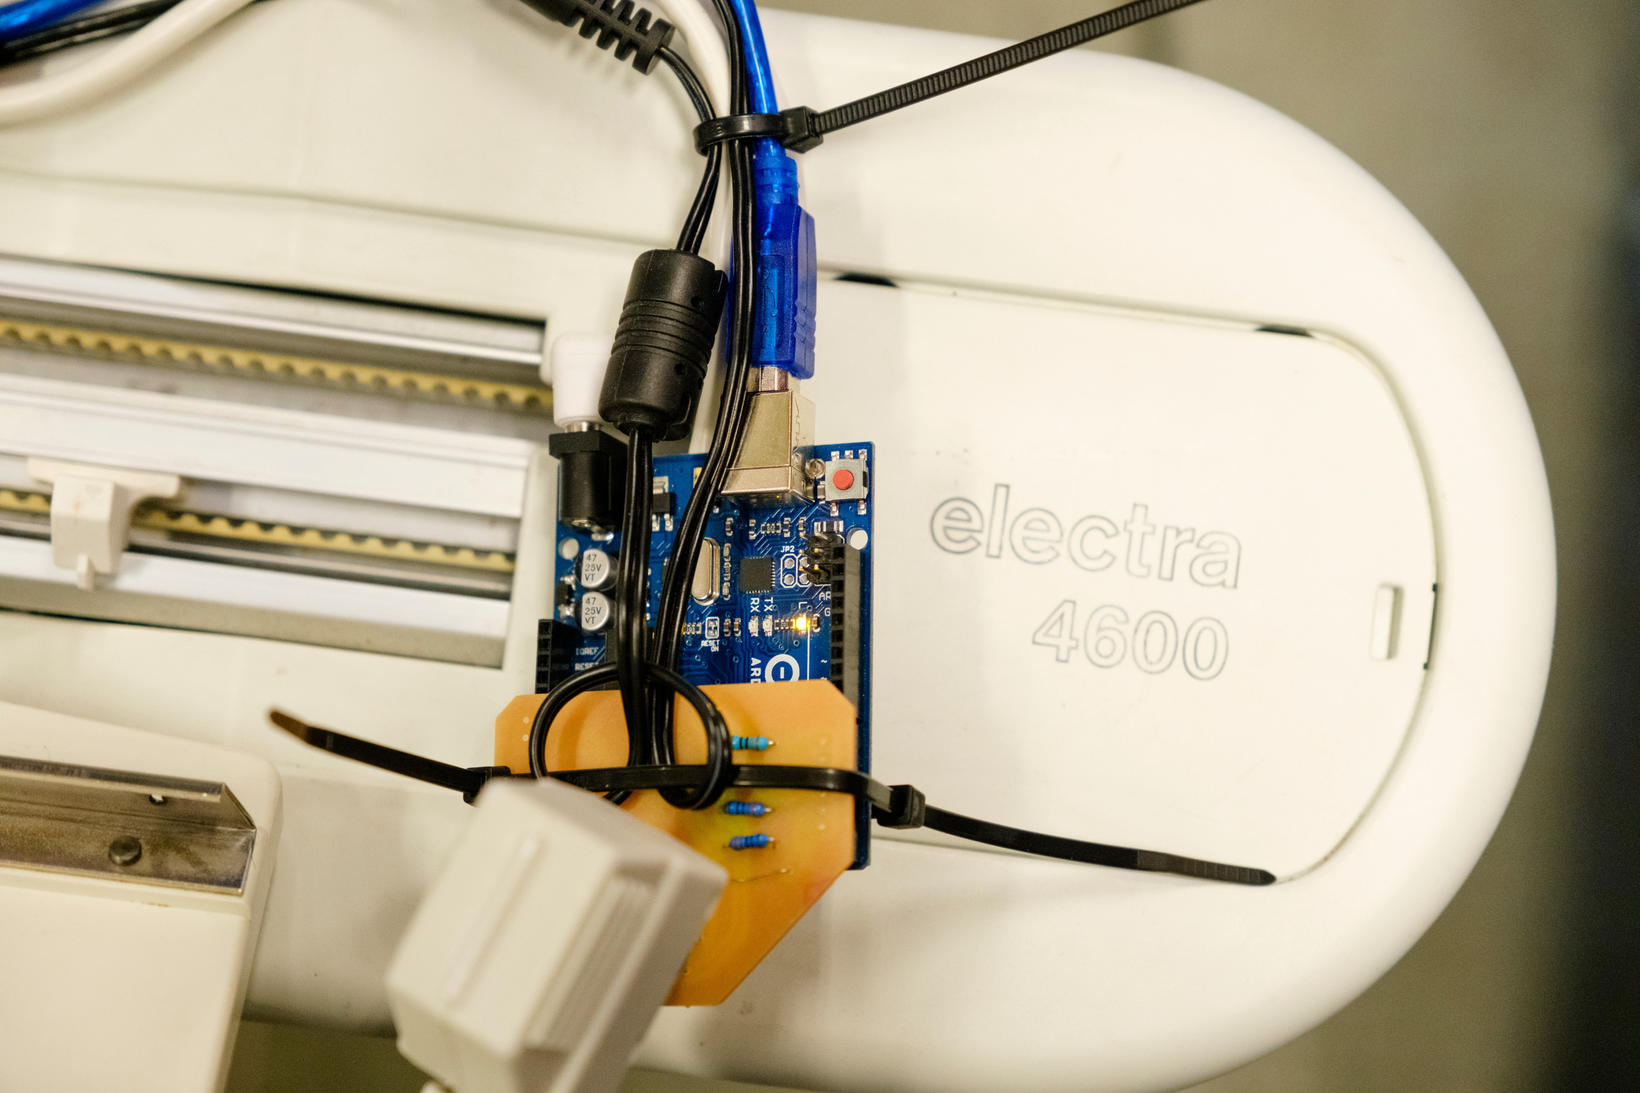
\includegraphics[width=0.5\linewidth]{myndir/elli/electra4600.jpg}
    \caption{\textit{Arduino} örtölva tengd við DIN-6 tengi á \textit{Passap E6000} - \textit{mbl.is/Kristinn Magnússon}}
    \label{fig:arduino}
\end{figure}
Það eru í raun tvö tilvik sem geta átt sér stað. Annaðhvort eru þeir í sömu stöðu eða í sitthvorri. Ef að aflestur ljósskynjara við breytingu á þeim sem er tendgur í pinna 2 er sú sama þá er við á leiðinni til hægri. Ef að þeir gefa sitthvort gildið þá erum við á leiðinni til vinstri. Örtölvan er því með innvortis teljara sem hækkar í gildi þegar aflesturinn er sá sami og lækkar þegar þeir gefa sitthvort gildið.
\begin{figure}[H]
    \centering
    \begin{tikzpicture}[auto, node distance=2cm, >=latex']
        \node [rectangle, draw, align=center] (arduino) {\textit{Arduino} örtölva};
        \node [rectangle, draw, align=center, right=4cm of arduino] (tlva) {tölva \\ keyrir stýringu};
        \node [rectangle, draw, align=center, below=4cm of arduino] (sled) {Sleði/Lás};
        \node [below=1cm of sled] (magnets) {};
        \node [left=1cm of sled] (light) {};
        \node [align=center, above=1cm of arduino] (power) {Spennubreytir};
        \node [rectangle, draw, align=center, above=1cm of tlva] (net) {Stjórnanda\\ vefviðmót};
        \node [align=center, below=1cm of tlva] (gagnagrunnur) {gagnagrunnur};
        \node [rectangle, draw, align=center, below=1cm of gagnagrunnur] (opid) {Opið\\ vefviðmót};
        \draw[-] (sled) edge[dotted, right] node[rotate=-90, above] {} (magnets)
                (sled) edge[dotted, right] node[rotate=-90, above] {} (light)
        
        
        ;
        \draw[->] 
(arduino) edge[dash dot, bend left] node[above] {\texttt{R} $\vee$ \texttt{L}} (tlva)
(tlva) edge[dash dot, bend left] node[below] {`\{byrjun\}\{munstur\}'} (arduino)
          (sled) edge[bend right] node[rotate=90, below] {lágur} (arduino)
          (sled) edge[bend right] node[rotate=90, above] {hár} (arduino)
                    (arduino) edge[->, bend right] node[align=center, rotate=90, below] {lágur} (sled)
          (arduino) edge[->, bend right] node[align=center, rotate=90, above] {hár} (sled)
          (power) edge[dashed,left] node[above] {} (arduino)
          (arduino) edge[dashed, left] node[left] {} (sled)
          (net) edge[<->,thick, dash dot dot] node[left] {} (tlva)
                    (gagnagrunnur) edge[<->,thick, dash dot dot] node[left] {} (tlva)
              (opid) edge[<->,thick, dash dot dot] node[left] {} (gagnagrunnur)

        ;

                \node[draw, rectangle, anchor=north west] at (2, -4) {
        \begin{tikzpicture}[x=1cm, y=0.8cm]
            \draw[thick] (0,0) -- (1,0) node[right] {5V};
             \draw[thick, dashed] (0,-0.5) -- (1,-0.5) node[right] {12V};
            \draw[thick, dash dot] (0,-1) -- (1,-1) node[right] {USB serial};
                        \draw[thick, dash dot dot] (0,-1.5) -- (1,-1.5) node[right] {Vefbeiðnir};
        \end{tikzpicture}};
    \end{tikzpicture}
    \caption{Kerfismynd af nýja stjórnborðið}
    \label{fig:newConsole}
\end{figure}
Nýja stýringin sem kemur í stað gamla stjórnborðsins hefur tvo meginliði örtölvuna og stýringin sem er keyrð á tölvu, sjá mynd \ref{fig:newConsole}. 
\begin{enumerate}
    \item \textbf{\textit{Arduino} örtölva} \begin{itemize}
        \item Sér um samskipti við sleðann með tengingu í gegnum DIN-6 tengi. Fær þaðan lestur af ljósskynjurum og stjórn á seglum. 
        \item Þegar skynjarinn sem er tengdur í pinna númer tvo breytir um gildi fer í gang truflun á kóðanum sem athugar um leið stöðuna á hinum ljósskynjaranum. Útfrá því fáum við út hvaða átt við erum að fara í. \begin{enumerate}
            \item Ef við fáum sitthvort gildið erum við að fara til vinstri. Teljari telur niður um einn.
            \item Ef við fáum sama gildið erum við að fara til hægri. Teljari telur upp um einn.
        \end{enumerate}
        \item Út frá innri teljaranum vitum við nákvæma staðsetningu sleðans á nálarbeðinu, svo lengi sem hann er tekinn útaf nálarbeðinu og setur aftur inná í hvert skipti sem örtölvan er endurræst/endurtengd.
        \item Örtölvan er skrifuð í C++ og hefur vigur með lengdina 179, eitt gildi fyrir hverja nál af nálarbeðinu. Það eru tvær aðrar breytur sem sjá um munstrin. Það er upphafs punktur og lengd munsturs. Grunngildin fyrir þau eru -10 og 10.
        \item Skilaboðin sem að \textit{Arduino} örtölvan sendir frá sér eru tvennskonar.
        \begin{enumerate}
            \item Ef að sleðin er vinstra megin við upphafs punktinn, teljari hefur gildi minna en upphafspunktsgildið. Þá er strengurinn \texttt{L} sendur yfir serial samskipti. 
            \item Ef að sleðin er hægra megin við punktinn sem er í fjarlægð lengd munstursins frá upphafspunktinnum, teljarinn hefur gildi sem er hææra en upphafspunktagildið lagt saman við lengd munstursins. Þá er strengurinn \texttt{R} sendur yfir serial samskipti.
        \end{enumerate}
        \item Þegar engin truflun á sér stað í keyrslu \textit{Arduino} örtölvunar þá ítrar hún fall sem athugar hvort einhver skilaboð hafi komið inn yfir serial tengi. Ef þau hafa komið inn, eru á strengjaformi sem hefur fleiri ein 3 stök þá er hann lesin sem staðlaður munsturs strengur. Þeir eru á forminu formerki serm er plús eða mínus. Síðan eru tveir tölustafir sem geta tekið gildi frá \texttt{01} upp í \texttt{90}. Þá loks kemur upp munstrið sem á að prjóna næstu umferð. Strengurinn hefur núll fyrir hverja nál sem á að prjóna lykkju.
        \begin{table}[H]
            \centering
	\begin{tabular}{|c|c|c|c|c|c|c|c|c|c|c|}
		\hline
		\multicolumn{1}{|c|}{\textbf{Formerki}} & \multicolumn{2}{c|}{\textbf{Upphafspunktur}} & \multicolumn{7}{c|}{\textbf{Munstur}} \\ 
		\hline
		- & 0 & 5 & 0 & 0 & 1 & 1 & 0 & 0 & 1 \\ 
		\hline
		\end{tabular}
            \caption{Sýnidæmi um löglegan munsturs sreng í serial samskiptum.}
            \label{tab:MunsturStrengur}
        \end{table}
        Formerkið gefur til kynna hvort megin við miðju nálarbeðsins munstrið á að byrja og upphafspunkturinn er númer nálar sem munstrið byrjar frá. Munstrið er alltaf skrifað frá vinstri til hægri.
    \end{itemize}
    \item \textbf{Tölvan sem keyrir stýringuna}
    Á vélinni þarf að vera uppset Node.js 20+, tenging með usb tengi við \textit{Arduino} örtölvuna.
    \begin{itemize}
        \item Stýringin sér um að geyma öll fylkin í heild sinni og matreiðir þá til \textit{Arduino} örtölvunar á réttu formi.
        \item Stýringin er alltaf að bíða eftir skilaboðum frá \textit{Arduino} örtölvunni. Þegar hún fær streng frá örtölvunni yfir serial samskipti athugar hún fyrst hvort það sé munstur að bíða eftir því að fara í vinnslu. Ef svo er þá er sía sem athugar ýmislegt en megin atriðið er hvort að næsta lína úr fylkinu sé oddatala eða ekki. \begin{enumerate}
            \item \texttt{L} sækir einungis næstu línu úr fylkinu ef númerlínunar er slétt. Sléttar tölur eru stilltar frá vinstri til hægri, hækkandi númer nála á nálarbeði. Þær eru síðan prjónar í öfuga átt.
            \item \texttt{R} sækir einungis næstu línu úr fylkinu ef númerlínunar er oddatala. Stilling og prjónun er í öfuga átt við \texttt{L}.
        \end{enumerate}
        \item Þegar munstur er senda á stýringuna er annað hvort:
        \begin{enumerate}
            \item Ekkert munstur í bið. Munstrið sett í minni og í vinnslu umleið.
            \item Munstur í vinnslu/bið og þá er nýja munstrinn bætt aftast í röðina.
        \end{enumerate}
        \item Stýringin hefur stjórnenda vefviðmót sem gefur notanda stýringar möguleika, eyða út munstrum, breyta upphafsnál o.s.frv. ásamt grafík sem sýnir núverandi stöðu vélarinar. Þar er hægt að sjá hvaða munstur er verið að stilla, hvað var stillt og hvað verður stillt næst.
        \item Stýringin tekur við munstrum í gegnum netbeiðnir, þær þurfa að innihalda upphafspunkt og munstursfylki. Munstursfylkin geta innihaldið tölugildi frá 0 til 4, eitt gildi fyrir hvern lit. Stýringin sér um að þýða fylkið og breytir öllum núllum í einn og öllum gildum í 0. Þá eru það gildin sem eru prjónuð.
        \item Bætt var við stýringar möguleika sem sækir munstur úr gagnagrunni ef ekkert munstur er í vinnslu eða bið.
        \item     \textbf{Opið vefviðmót}
    tekur við texta beiðnum frá notendum. Notfærir sér netsamskipti til að búa til mynd úr textanum með hjálp gervigreindar. Þá er bakgrunninn staðlaður. Myndin er síðan breytt í munstursfylki og vistað í gagnagrunni.       
    \end{itemize}
\end{enumerate}
\subsubsection{Stýring á mótor}
Passap vélarnar fóru í gegnum miklar framfarir á þeim tíma sem þær voru í framleiðslu. Upphaflega þurfti notandinn að stilla munstrinn sjálfur og færa sleðann. Snemma var komin lausn með mótor og einföldum breytingum á munstri með seglum. Mótorarnir breytust einnig og voru fyrstu stýrðir með fótapedölum. Síðan kom takkastýring sem bauð notendum á að stýra mótornum á þægilegri máta. Þetta hélt áfram lengi þar til \textit{Passap E6000} kom út með stjórnborðið sem gat gert allskyns munstur með hjálp innbyggðrar \textit{Form} tölvu. Hann hinsvegar tók yfir stjórn á tökkunum og þurfti í þeirri útfærslu að hafa stjórnborðið tengt og kveikt til að geta ýtt á takkanna. Þegar vélin var tekin í sundur kom í ljós að rafrásirnar af eldri útgáfunum eru enn til staðar og hægt er að tengja framhjá stjórnborðinu. Þá eru takkarnir aftur starfhæfir án stjórnborðsins. Takkastýringin er skýr og einföld.

\textbf{Til að stýra mótornum með \textit{Arduino} örtölvu} er hægt að nota 7407N kubb í einfaldri rafrás sem tengir pinna frá örtölvunni við stýri pinna á 7407N og pinanna sem er stjórnað við rafrásir hvers takka. Takkarnir virka þannig að þeir eru alltaf með $5V$ straum á \textit{high} og þegar hann er tengdur í \textit{ground} er takkurinn virkur. 7407N hermir eftir því. Það er pláss fyrir skipanir í \textit{Arduino} kóðanum fyrir skipanir á strengjaformi sem hafa 3 stafi eða færri. 
Útfærsla á rafrás er hægt að sjá á mynd ##. 
Í kóða er nú þegar skipunin \texttt{s} notuð til að slökkva og kveikja á mótor.

\subsection{Sjálfvirk mynsturgerð}
\subsubsection{Mynstur unnin til að senda á vél}
Byrjað var á því að skrifa kóða sem tekur fylki af tölum sem táknar mynd sem á að prjóna og kemur því yfir á rétt form til að senda á prjónavélina. Litirnir geta verið í mesta lagi fjórir og inniheldur hvert munstur sem sent er á vélina þar með heiltölurnar $1$, $2$, $3$ og $4$ eftir því með hve mörgum litum á að prjóna. Sérhver $1$ í munstrinu táknar eina lykkju sem á að prjóna með lit eitt, $2$ táknar lykkjur sem prjóna á með lit t o.s.frv. Talan $0$ táknar óprjónaðar lykkjur. 

Vélin prjónar með aðeins einum lit í einu og prjónar tvær umferðir áður en skipt er um lit. Ef prjónað er með fjórum litum tekur því hver lína í munstur fylkinu átta umferðir í vélinni. Skrifað var fall sem tekur inn fylki af tölum og aðskilur tölurnar í mismunandi lista þar sem fyllt er upp í með núllum og þ.a. hver listi kemur tvisvar sinnum fyrir (þar sem í fyrst fer sleðinn frá hægri til vinstri og svo fer sleðinn vinstri til hægri). 

\textbf{Dæmi}: Ef gefið er eins línu munstrið $$[1,2,2,3,4]$$ skilar fallið lista af listum: 
\[
\left[
\begin{array}{c}
\left[1, 0, 0, 0, 0\right], \left[1, 0, 0, 0, 0\right], \\
\left[0, 2, 2, 0, 0\right], \left[0, 2, 2, 0, 0\right], \\
\left[0, 0, 0, 3, 0\right], \left[0, 0, 0, 3, 0\right], \\
\left[0, 0, 0, 0, 4\right], \left[0, 0, 0, 0, 4\right]
\end{array}
\right]
\]
Á mynd \ref{fig:litid_prjon} má sjá hvernig einfaldri mynd er lýst með fylki af tölum og svo hvernig prjónamunstrið sem sent er á vélina lítur út ef prjóna á myndina.

\begin{figure}
    \centering
    
\includegraphics[height=.3\textheight]{myndir/snaeja/litid_prjon_fyrir.png}
    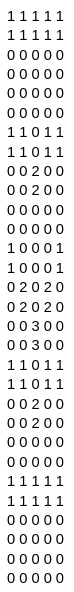
\includegraphics[height=.3\textheight]{myndir/snaeja/litid_prjon_separated.png}
    \caption{Til hægri má sjá einfalt prjónamunstur í þremur litum þar sem hver heiltala táknar eina lykkju í ákveðnum lit. Til vinstri hvernig sama munstur lítur út áður en það er sent á vélina.}
    \label{fig:litid_prjon}
\end{figure}

\subsubsection{Íslenska Sjónabókin nýtt í mynsturgerð}
Íslenska Sjónabókin inniheldur útsaums munstur úr þeim sjónabókum sem varðveist hafa á Íslandi. Með \textit{Íslensku Sjónabókinni} fylgir geisladiskur með öllum þeim síðum af munstrum sem í henni eru. Skrárnar eru ýmist á \texttt{.pdf} eða \texttt{.eps} formi og henta illa til að vinna með í tölvu. Til að nýta munstrin og senda þau á prjónavélina þurfti að koma þeim á annað og betra stafrænt form. Langflest munstrin í bókinni eru í tveimur litum þ.e. kross og ekki kross og því var einskorðað á þau í þessum hluta verkefnisins.

Skrifaður var kóði sem settur var á GitHub\footnote{Kóðinn og mynstrin má finna á \url{https://github.com/HiDefTextiles/Sjonabok}.} þ.a. hver sem getur sótt kóðann og notað mynstrin á handhægara formi. Kóðinn virkar þannig að hver \texttt{.eps} skrá er sótt og sett í grátóna fylki í Python. Fylkinu er svo skipt í núll og einn þannig að hver pixill sem er yfir ákveðinn þröskuld af dökkum gráum er látinn vera svartur ($1$) og restin er sett sem hvítur($0$). Síðan eru rúðustrikuðu línurnar fundnar og innan hvers reits ef hlutfall svartra pixla er yfir $0.5$ er litið á sem svo að kross sé inni í reitinum. Þessum upplýsingum er svo safnað saman í nýtt fylki þar sem $1$ stendur fyrir kross og $0$ engan kross. Öllu auka plássi fyrir utan munstrið er síðan hent og fylkið vistað á tveimur skráarsniðum, texta sniði og \texttt{.png} sniði. Texta skránum er einfalt að hlaða inn í fylki til að nota síðar og þægilegra er að skoða munstrin á \texttt{.png} sniði. Á mynd \ref{fig: sjonabok_munstur} má sjá hvernig munstur lítur út eftir vinnslu. 


\begin{figure}
    \centering
    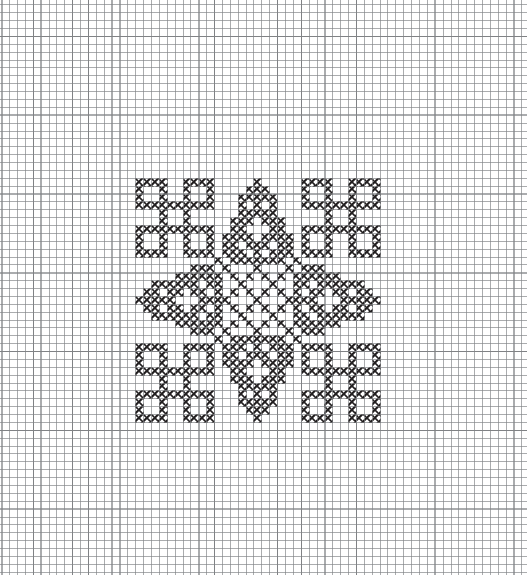
\includegraphics[height=.3\textheight]{myndir/snaeja/sjonabok_before.png}
    
\includegraphics[height=.3\textheight]{myndir/snaeja/sjonabok_after.png}
    \caption{Til hægri má sjá munstur úr \textit{Íslensku Sjónabókinni} í \texttt{.eps} skrá. Til vinstri hvernig sama munstur lítur út eftir vinnslu á \texttt{.png} formi.}
    \label{fig: sjonabok_munstur}
\end{figure}

Í sumum skrám er fleira ein eitt munstur að finna. Til að geta nýtt þau þarf að aðskilja þau. Borða er einfalt að aðskilja þar sem þeir aðskiljast alveg einungis lárétt eða lóðrétt. Önnur munstur og stafróf aðskiljast á flóknari máta og var útfærlsa af DFS nýtt til að aðskilja þau. Aðskilin munstur eru svo vistuð sér þ.a. ein síða af munstrum fara í sömu möppu. Einnig var skrifaður kóði sem finnur endurtekningar í munstri og geymir þá minnstu endurtekninguna.

Skrifuð voru nokkur föll fyrir munsturgerð í Python footnote {Kóða fyrir mynsturgerðina má finna á \url{https://github.com/snaefi/mynsturgerd}.}. Eitt af þeim var fall sem breytir myndum (\texttt{.jpg} eða \texttt{.png}) í prjónamynstur. Fallið tekur inn vísun á myndaskrá, hversu margar lykkjur munstrið á að vera og fjölda lita. Fallið gráskalar myndina, fækkar pixlum í samræmi við fjölda lykkja og notar síðan Floyd-Steinberg reikniritið til að fækka litum \cite{FloydSteinberg}. Fallið skilar svo fylki af heiltölum á bilinu $1$ til $4$ þar sem $1$ táknar ljósustu pixlana á grátóna bilinu og hæsta talan þá dekkstu. Sökum þess hvernig Floyd-Steinberg reikniritið virkar að ef bakgrunnur einhverrar myndar er aðeins í einum lit endar hann oft á að innihalda staka pixla í dekkri lit eftir að því er beitt á myndina. Því var skrifað reiknirit sem tekur svoleiðis staka pixla og breytir þeim í sama lit og aðalbakgrunnslitinn. Við gerð þessa reiknirits var \textit{flood fill} reikniritið nýtt \cite{flood-fill}.

Önnur föll sem nýta sjónabókamunstrin voru einnig skrifuð. Eitt þeirra bætir við borða umhverfis prjónamunstur eftir óskum notendans (mynd \ref{fig: sjonabok_bordi}). Annað gerir kleift að skrifa texta með sjónabókar leturgerðum eins og sjá má á mynd \ref{fig:hallo_heimur}. Textinn getur ýmist verið  miðjaður eða vinstri jafnaður. Skrifað var fall sem bætir við sjónabókarmunstri sem bakgrunni við munsturfylki (mynd \ref{fig:raggajóns}). Það fall nýtir \textit{flood fill} reikniritið \cite{flood-fill}. Fallið var útfært þannig að ef mynd er prjónuð og bakgrunnur bættur við hana getur næsta mynd sem er prjónuð einnig haft sama bakgrunn og þannig að bakgrunnarnir renna saman í einn heildstæðan bakgrunn þ.e. ekki sjást skil í bakgrunninum á milli myndanna tveggja.

\begin{figure}[p]
    \centering
    \begin{minipage}[b]{0.45\linewidth}
        \centering
        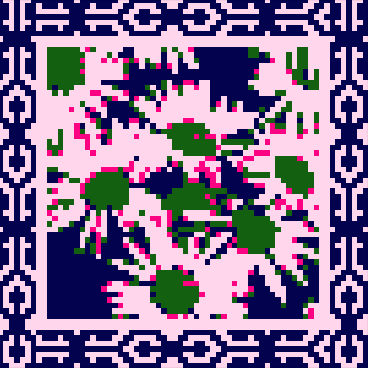
\includegraphics[width=.8\linewidth]{myndir/snaeja/bordi.png}
        \caption{Borða úr \textit{Íslensku Sjónabókinni} bætt við í kringum prjónamynstur. Prjónamynstrið er í 4 litum og kemur frá ljósmynd af baldursbrám.}
        \label{fig: sjonabok_bordi}
    \end{minipage}
    \hspace{0.05\linewidth} % Add space between the figures
    \begin{minipage}[b]{0.45\linewidth}
        \centering
        \includegraphics[width=\linewidth]{myndir/snaeja/raggajóns.png}
        \caption{Prjónamynstur af Ragnheiði Jónsdóttur með mynstur úr \textit{Sjónabók} sem bakgrunn.}
        \label{fig:raggajóns}
    \end{minipage}
\end{figure}

\begin{figure}[p]
    \centering
    
\includegraphics[width=0.5\linewidth]{myndir/snaeja/hallo_heimur.png}
    \caption{\textit{Halló heimur} prjónamynstur skrifað með letri úr \textit{Sjónabók}.}
    \label{fig:hallo_heimur}
\end{figure}

\subsubsection{Ókláruð verkefni}
Aðrar aðferðir voru prófaðar fyrir mynstur gerð. \textit{Wave Function Collapse} (WFC) reikniritið var sett upp með hnútum sem finna má á mörgum stöðum í \textit{Íslensku Sjónabókinni}. Ákveðið var þessi munsturgerð myndi ekki henta í hönnunarvinnuna að svo stöddu og því var ekki kafað dýpra ofan í WFC en á mynd \ref{fig:wfc} má sjá útkomu úr reikniritinu. Einnig var byrjað á að þróa aðferð sem litar munstur úr sjónabókinni sjálfvirkt í 3 til 4 litum. Sökum tímahraks tókst ekki að klára þá vinnu en var hún komin nokkuð áleiðis og mætti halda áfram með hana síðar.

\begin{figure}[p]
    \centering
    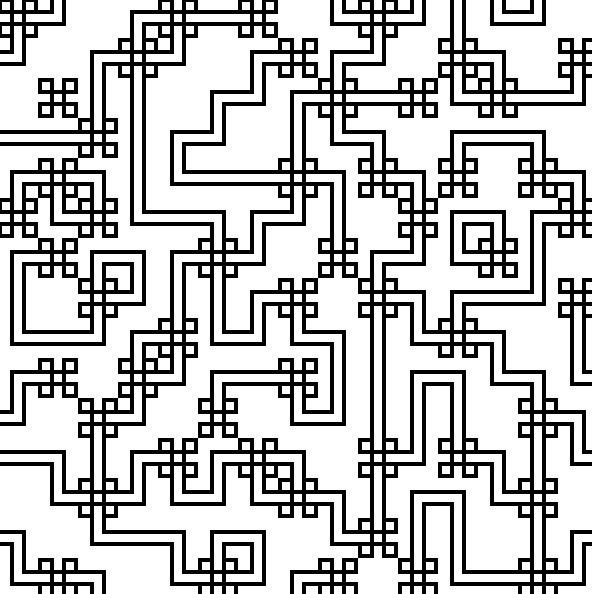
\includegraphics[width=0.5\linewidth]{myndir/snaeja/wfc.png}
    \caption{\textit{Wave Function Collapse} reikniritið notað til að búa til prjónamunstur. Hnúturinn í munstrinu finnst á mörgum stöðum í \textit{Íslensku Sjónabókinni} en dæmi um hann er á mynd \ref{fig: sjonabok_munstur}.}
    \label{fig:wfc}
\end{figure}

\subsection{Prjón- og hönnunarvinna}
Prjón og hönnun var unnin í nánu samstarfi tölvunarfræðinema og fatahönnuðar og lagði mesta áherslu á hugmyndir útfærsla, möguleika í prjóni auk þess að leggja áherslu á framleiðslu á vélprjóni á \textit{Passap 6000}. Með  samstarfinu varð niðurstaðan áhugaverðari og náði betur til hönnuða en ella. 

\subsubsection{Hlutverk fatahönnuðar}
Hlutverk fatahönnuðsins var því að veita fagurfræðilega leiðsögn frá sjónarhorni hönnuða. Afurðin var jafnvægi milli skapandi hönnunar, hagnýtra takmarkana vélarinnar og þess sem hægt var að kóða á þessum skamma tíma. 

Þar sem möguleikar uppfærðrar prjónavélar voru óljósir við upphaf verkefnisins var erfitt að sjá fyrir lokaútkomu í hönnun. Því var hönnunarferlið sífellt á breytingu en lagði áherslu á möguleikana í stað þess að einblína á loka útkomu hönnunar. 

\subsubsection{Hönnunarhugsun}
Hönnuður styður sig við hugmyndir hönnunar hugsunar (e. Design Thinking) sem gjarnan er kennd við hönnunardeild Stanford háskóla í Kaliforníu \cite{designthinking}.  Þau skilgreina 5 stig hönnunar:
\begin{enumerate}
    \item Samkennd (e. Empathize): hvers vegna er hönnunin mikilvæg,
    \item Þarfir (e. Define): þarfir afmarkaðar,
    \item Hugmyndir (e. Ideate): ýmsar aðferðir skoðaðar,
    \item Frumgerð (e. Prototype): hugmyndir afmarkaðar og að lokum
    \item Prófun (e. Test) en þar eru hugmyndir kynntar til þess að fá viðbrögð frá ólíkum aðilum.
\end{enumerate}
Hönnuður náði  4 stigum hönnunar enn sem komið er en næsta og jafnframt afurð síðasta stigsins verður kynnt á Hönnunarmars.

\subsubsection{Prjón með mörgum litum}
Prufað var að prjóna með tveimur litum og kóðinn nýttur til þess að senda á prjónavélina texta eða mynstur í tveimur litum, sjá myndir \ref{fig:peacock}-\ref{fig:repeat} af fyrstu prufum sumarsins. Með uppfærslu var hægt að prjóna með þremur litum og að lokum fjórum. Útkomurnar urðu sífellt áhugaverðari og flóknari. 

Misvel gekk þó að prjóna og í byrjun áttum við erfitt með að prjóna með 4 litunum. Þá voru prjónaðar 8 umferðir á aftara borðinu fyrir hverja eina umferð á því fremra. Þetta olli miklum vandræðum en með breyttu prjóni, sem aðeins prjónar aðra hverja lykkju að aftan gekk betur að nota alla fjóra litina. Þá  voru prjónaðar 4 umferðir að aftan fyrir hverja eina að framan. 
\subsubsection{Áskoranir og betrumbætur í prjóni}
Stöðugt var verið að betrumbæta kóðana sem auðveldaði fyrir okkur prjónið. Margar prufurnar voru prjónaðir með handafli en þegar líða fór á sumarið tók mótorinn loksins við. Ýmis mannleg mistök áttu sér stað og gleymist reglulega að passa að setja strekkjarana aftur á þegar búið var að laga það sem laga þurfti. Þetta olli því að garnið komst illa á nálarnar sem verður til þess að sleðinn festist. Einnig kom fyrir að sleðinn náði ekki að grípa í næsta lit og prjónaði því garnlaus, þar með er prjónið fellt af. Þá þurfti annað hvort að byrja að prjóna upp á nýtt eða hengja lykkjurnar aftur á, en sem betur fer kom þetta ekki oft fyrir. 
\subsubsection{Ferlið sem lærdómstól}
Ferlið í heild sinni var mjög persónulegt þar sem hver og ein prufa var mikilvægur partur og gaf okkur upplýsingar um hönnunina, kóðann og prjónið. Mistökin kenndu okkur og færðu okkur nær þeim möguleikum sem við getum náð fram í dag. Prufurnar stýrðu því hönnunarferlinu að miklu leiti og notaði hönnuður hönnunarmál sitt til þess að túlka prufurnar í mögulegum lokaútkomum. 
\subsubsection{Sjálfbærar lausnir og framtíðarfatnaður}
Þessi hönnun kemur til með að vera undirstaða fatnaðar sem verður gerður fyrir Hönnunarmas næsta vor. Hannaðar voru flíkur sem nýta þær prufur sem nú þegar hafa verið prjónaðar. Leitað var sjálfbærra lausna og lagt áherslu á að gera persónulega og einstaka hönnun sem eykur verðmætagildi hönnunarinnar. Nokkrar útfærslur af fatnaði má sjá á mynd \ref{fig:designproposal}.

\begin{figure}
    \centering
    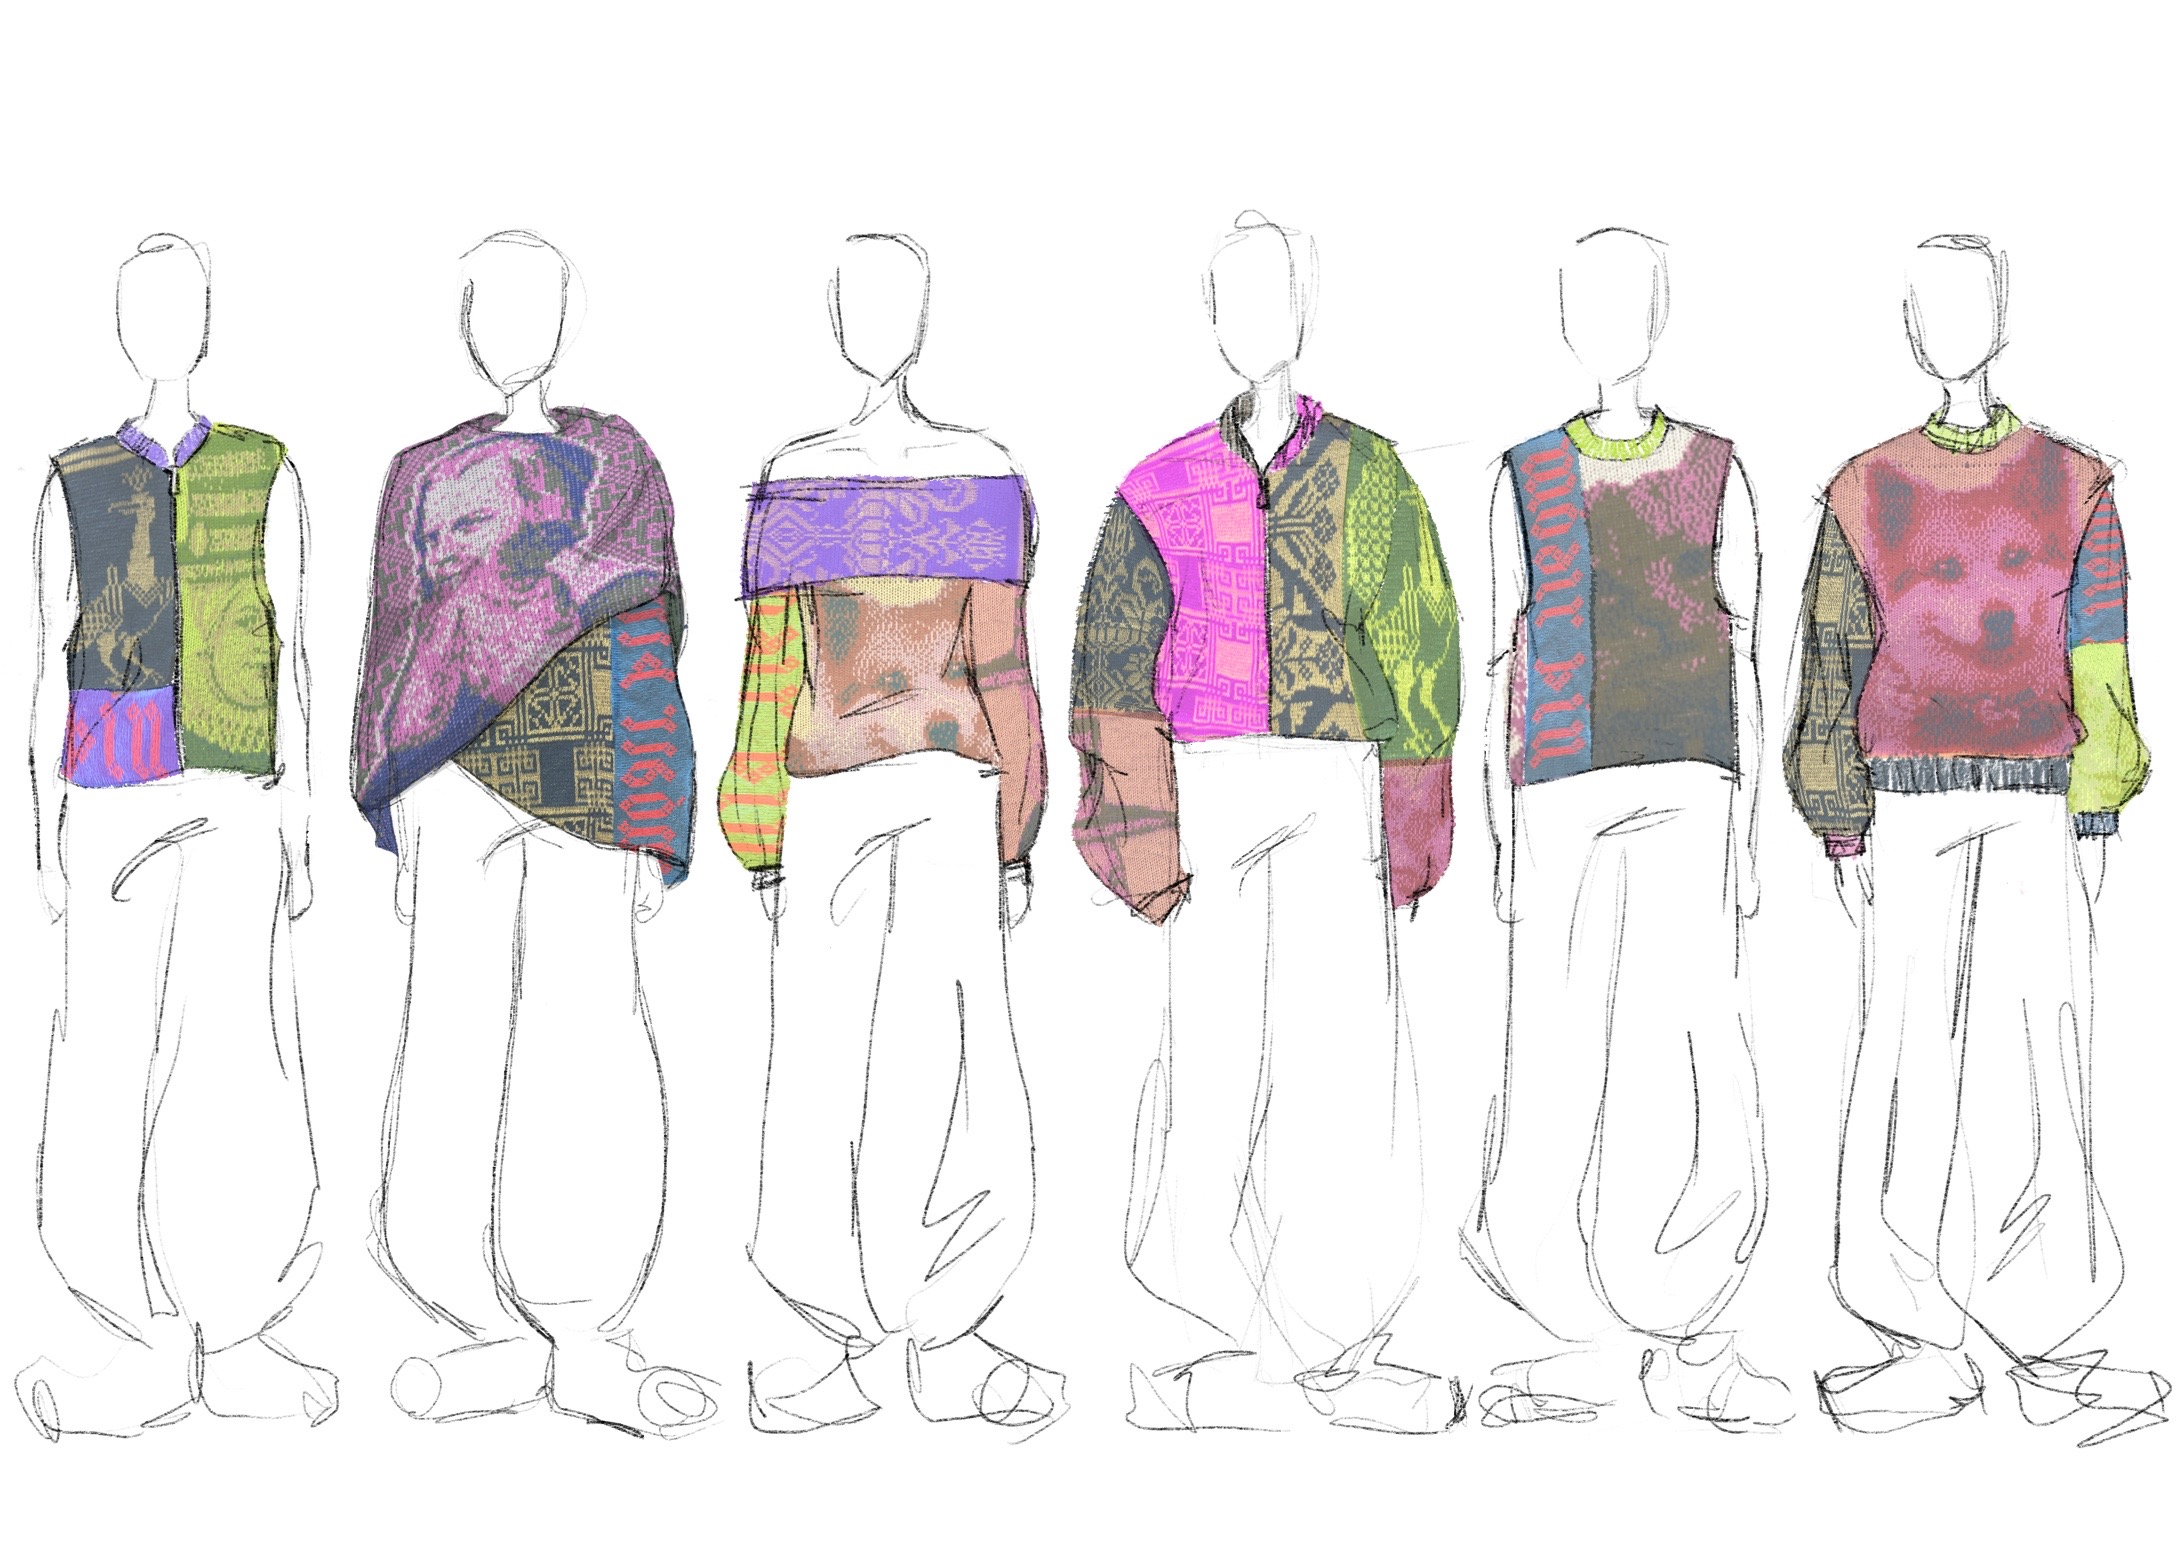
\includegraphics[width=\linewidth]{myndir/gisa/collection.JPG}
    \caption{Nokkrar útfærslur á fatnaði út frá prjónaprufum sumarsins.}
    \label{fig:designproposal}
\end{figure}

\subsubsection{Menningararfur og tenging við fortíðina}
Ragnheiður ,,yngri'' Jónsdóttir sem margir kannast eflaust við af 5.000kr seðlinum var mikil handverkskona og safnaði í sjónabók sem notuð var í mynstur í fyrsta kafla \textit{Íslenskrar sjónabókar} og er hún því áhrifamikil í menningararfi okkar Íslendinga. Á Þjóðminjasafni Íslands heillaðist hönnuður af henni og hennar mynstrum og ákváðum við því að heiðra framlag hennar með því að prjóna mynd af henni. Þessi prufa var byltingarkennd í ferlinu og má sjá mynd af henni, 50 lykkjur á breidd og aðra, 120 lykkjur á breidd á mynd \ref{fig:ragga:knit}. Í framhaldinu fórum við að blanda saman myndum og mynstrum og þannig tengja menningararf okkar inn í nútíma hönnun með því að blanda nútíð og fortíð saman. Hallgrímskirkja var ein þeirra eins og má sjá á mynd \ref{fig:hallgrimskirkja}. Náin samvinna tölvunarfræðinema og hönnuðar var lykilatriði í framvindu verkefnisins og býður upp á marga ókannaða möguleika. 

\begin{figure}[p]
    \centering
    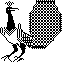
\includegraphics[height=.20\textheight]{myndir/thjms5898_246_0.png}
    \hspace{24pt}
    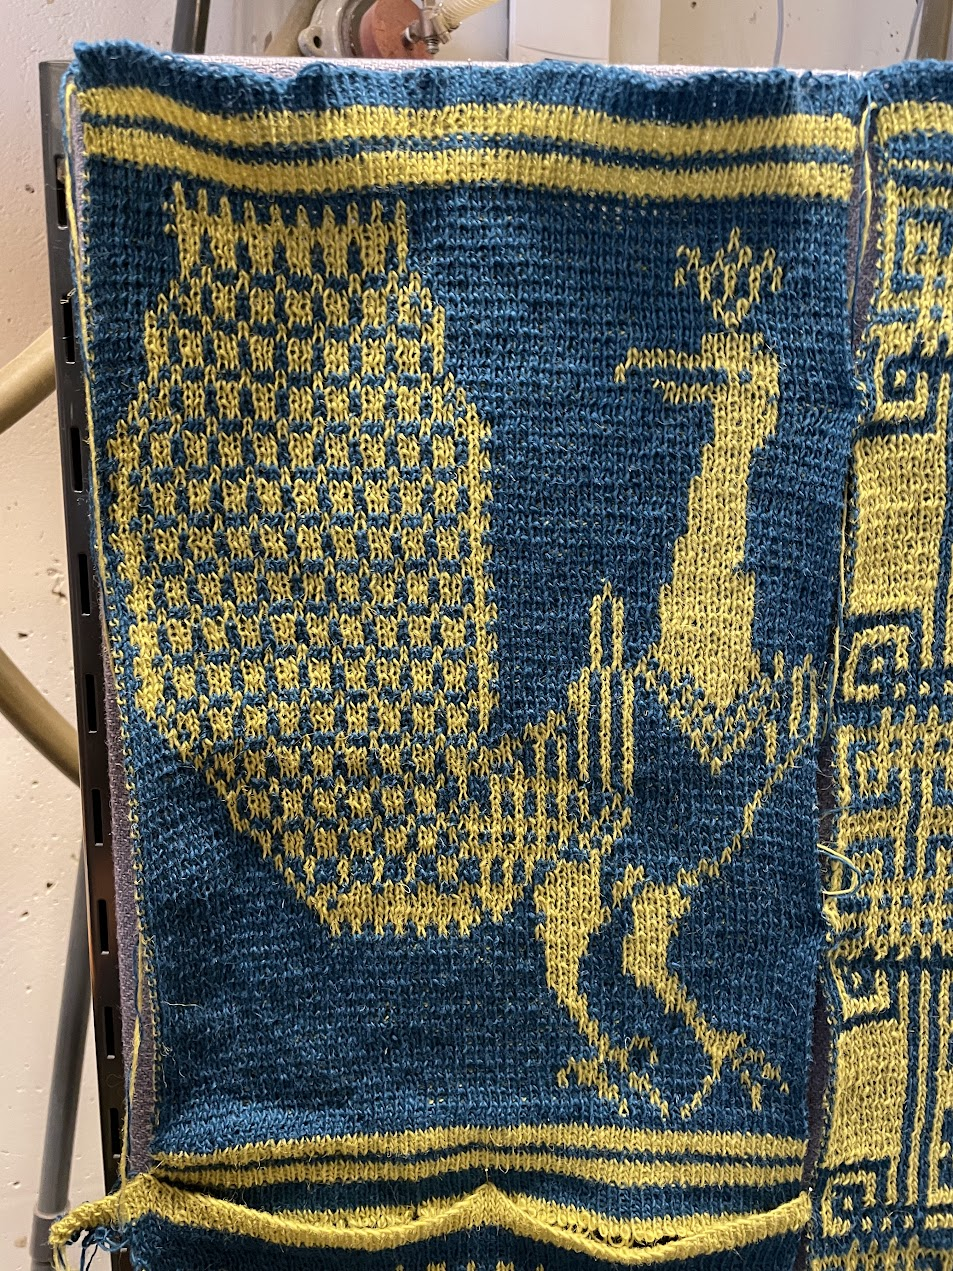
\includegraphics[height=.20\textheight]{myndir/peacock.jpg}
    \caption{Páfugl, bls. 246 í Sjónabók (Þjms. 5898)}
    \label{fig:peacock}
\end{figure}

\begin{figure}[p]
    \centering
    
\includegraphics[height=.20\textheight]{myndir/thjms5898_210.png}
    \hspace{24pt}
    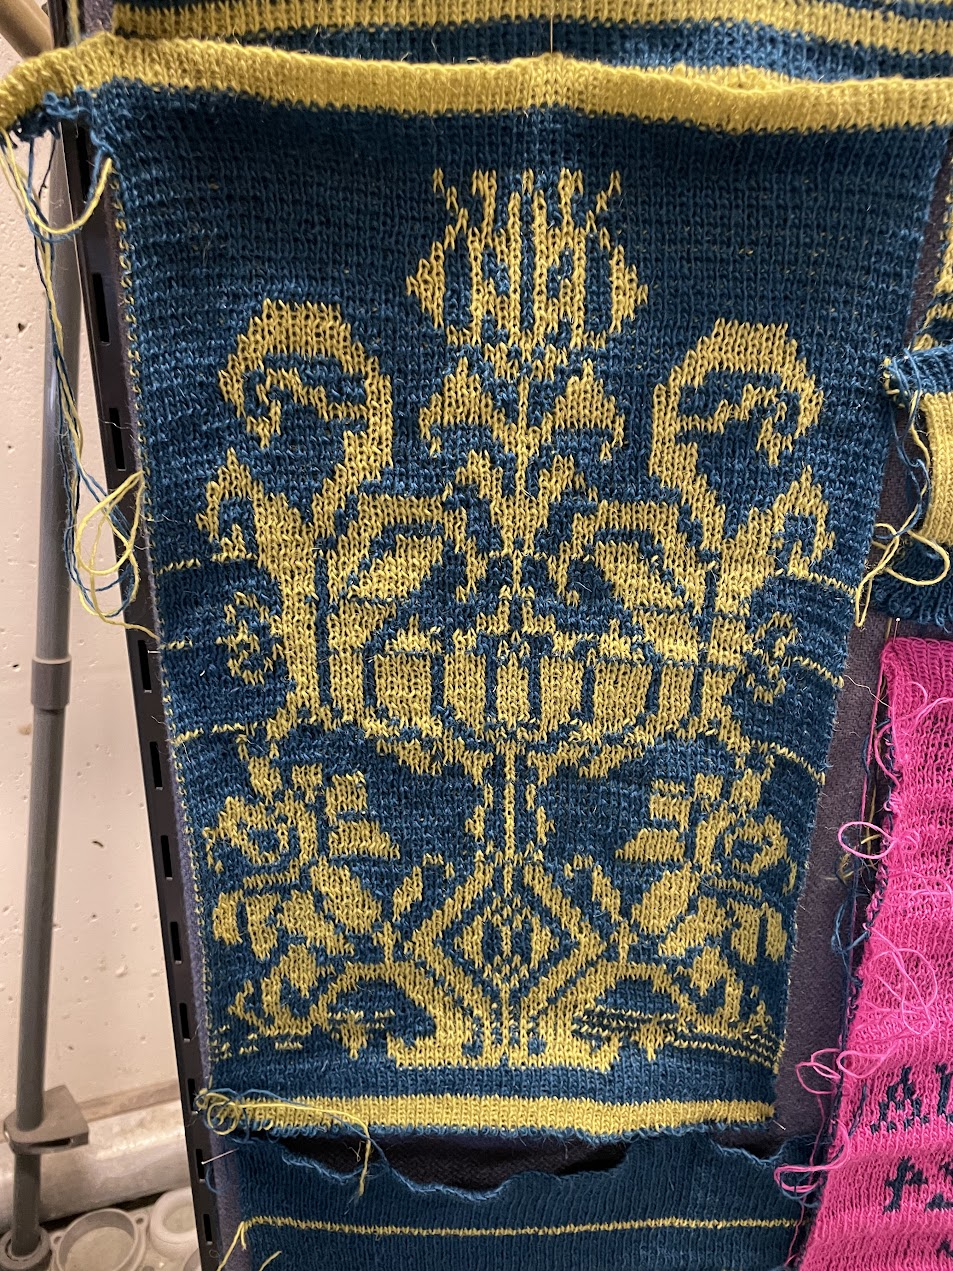
\includegraphics[height=.25\textheight]{myndir/flower.jpg}
    \caption{Blóm, bls. 210 í Sjónabók (Þjms. 5898)}
    \label{fig:flower}
\end{figure}

\begin{figure}[p]
    \centering
    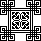
\includegraphics[height=.20\textheight]{myndir/thjms5898_268.png}
    \hspace{24pt}
    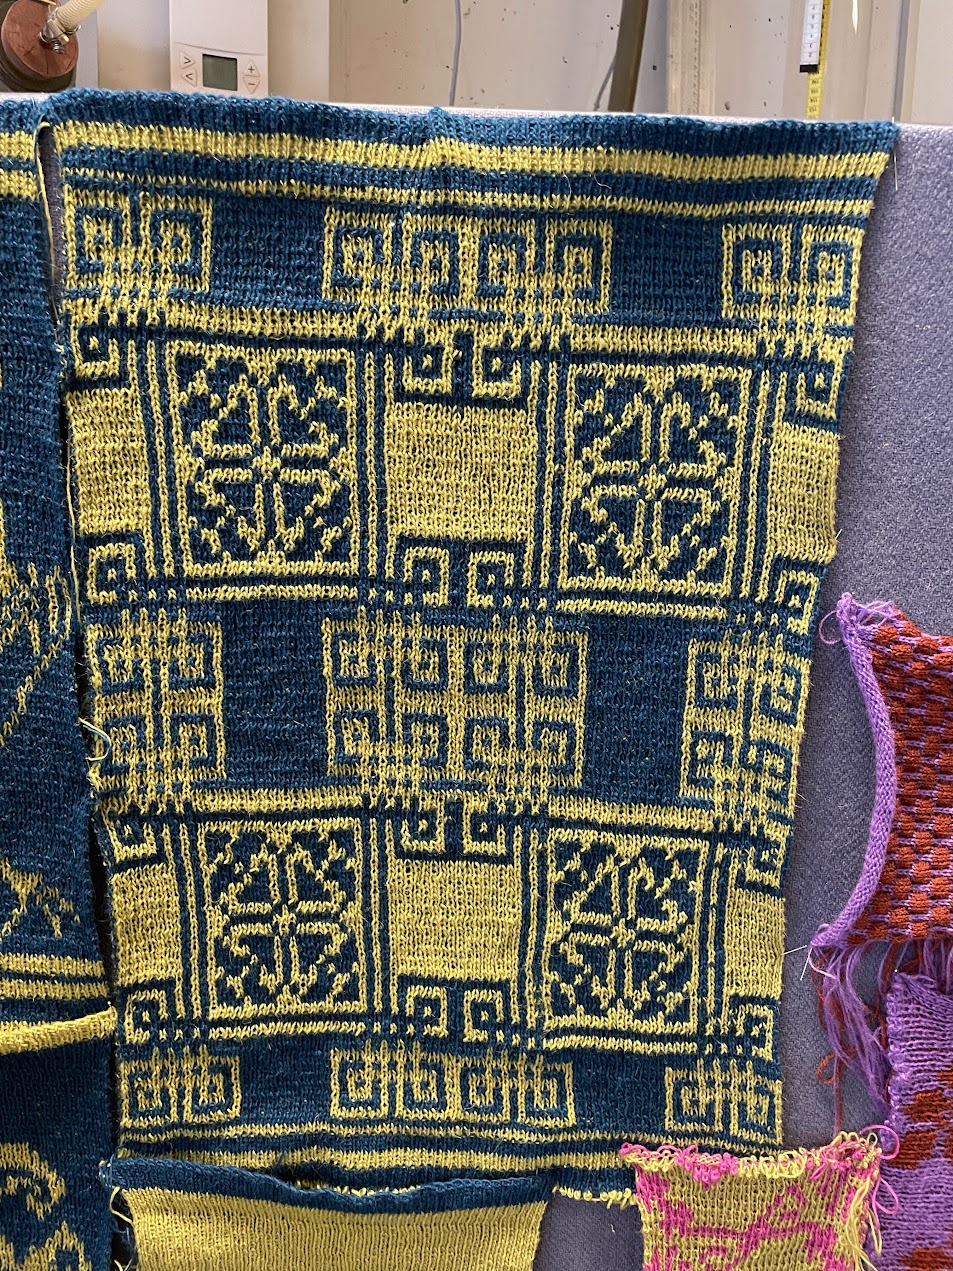
\includegraphics[height=.25\textheight]{myndir/repeat.jpg}
    \caption{Endurtekið mótif, bls. 268 í Sjónabók (Þjms. 5898)}
    \label{fig:repeat}
\end{figure}

\begin{figure}[p]
    \centering
    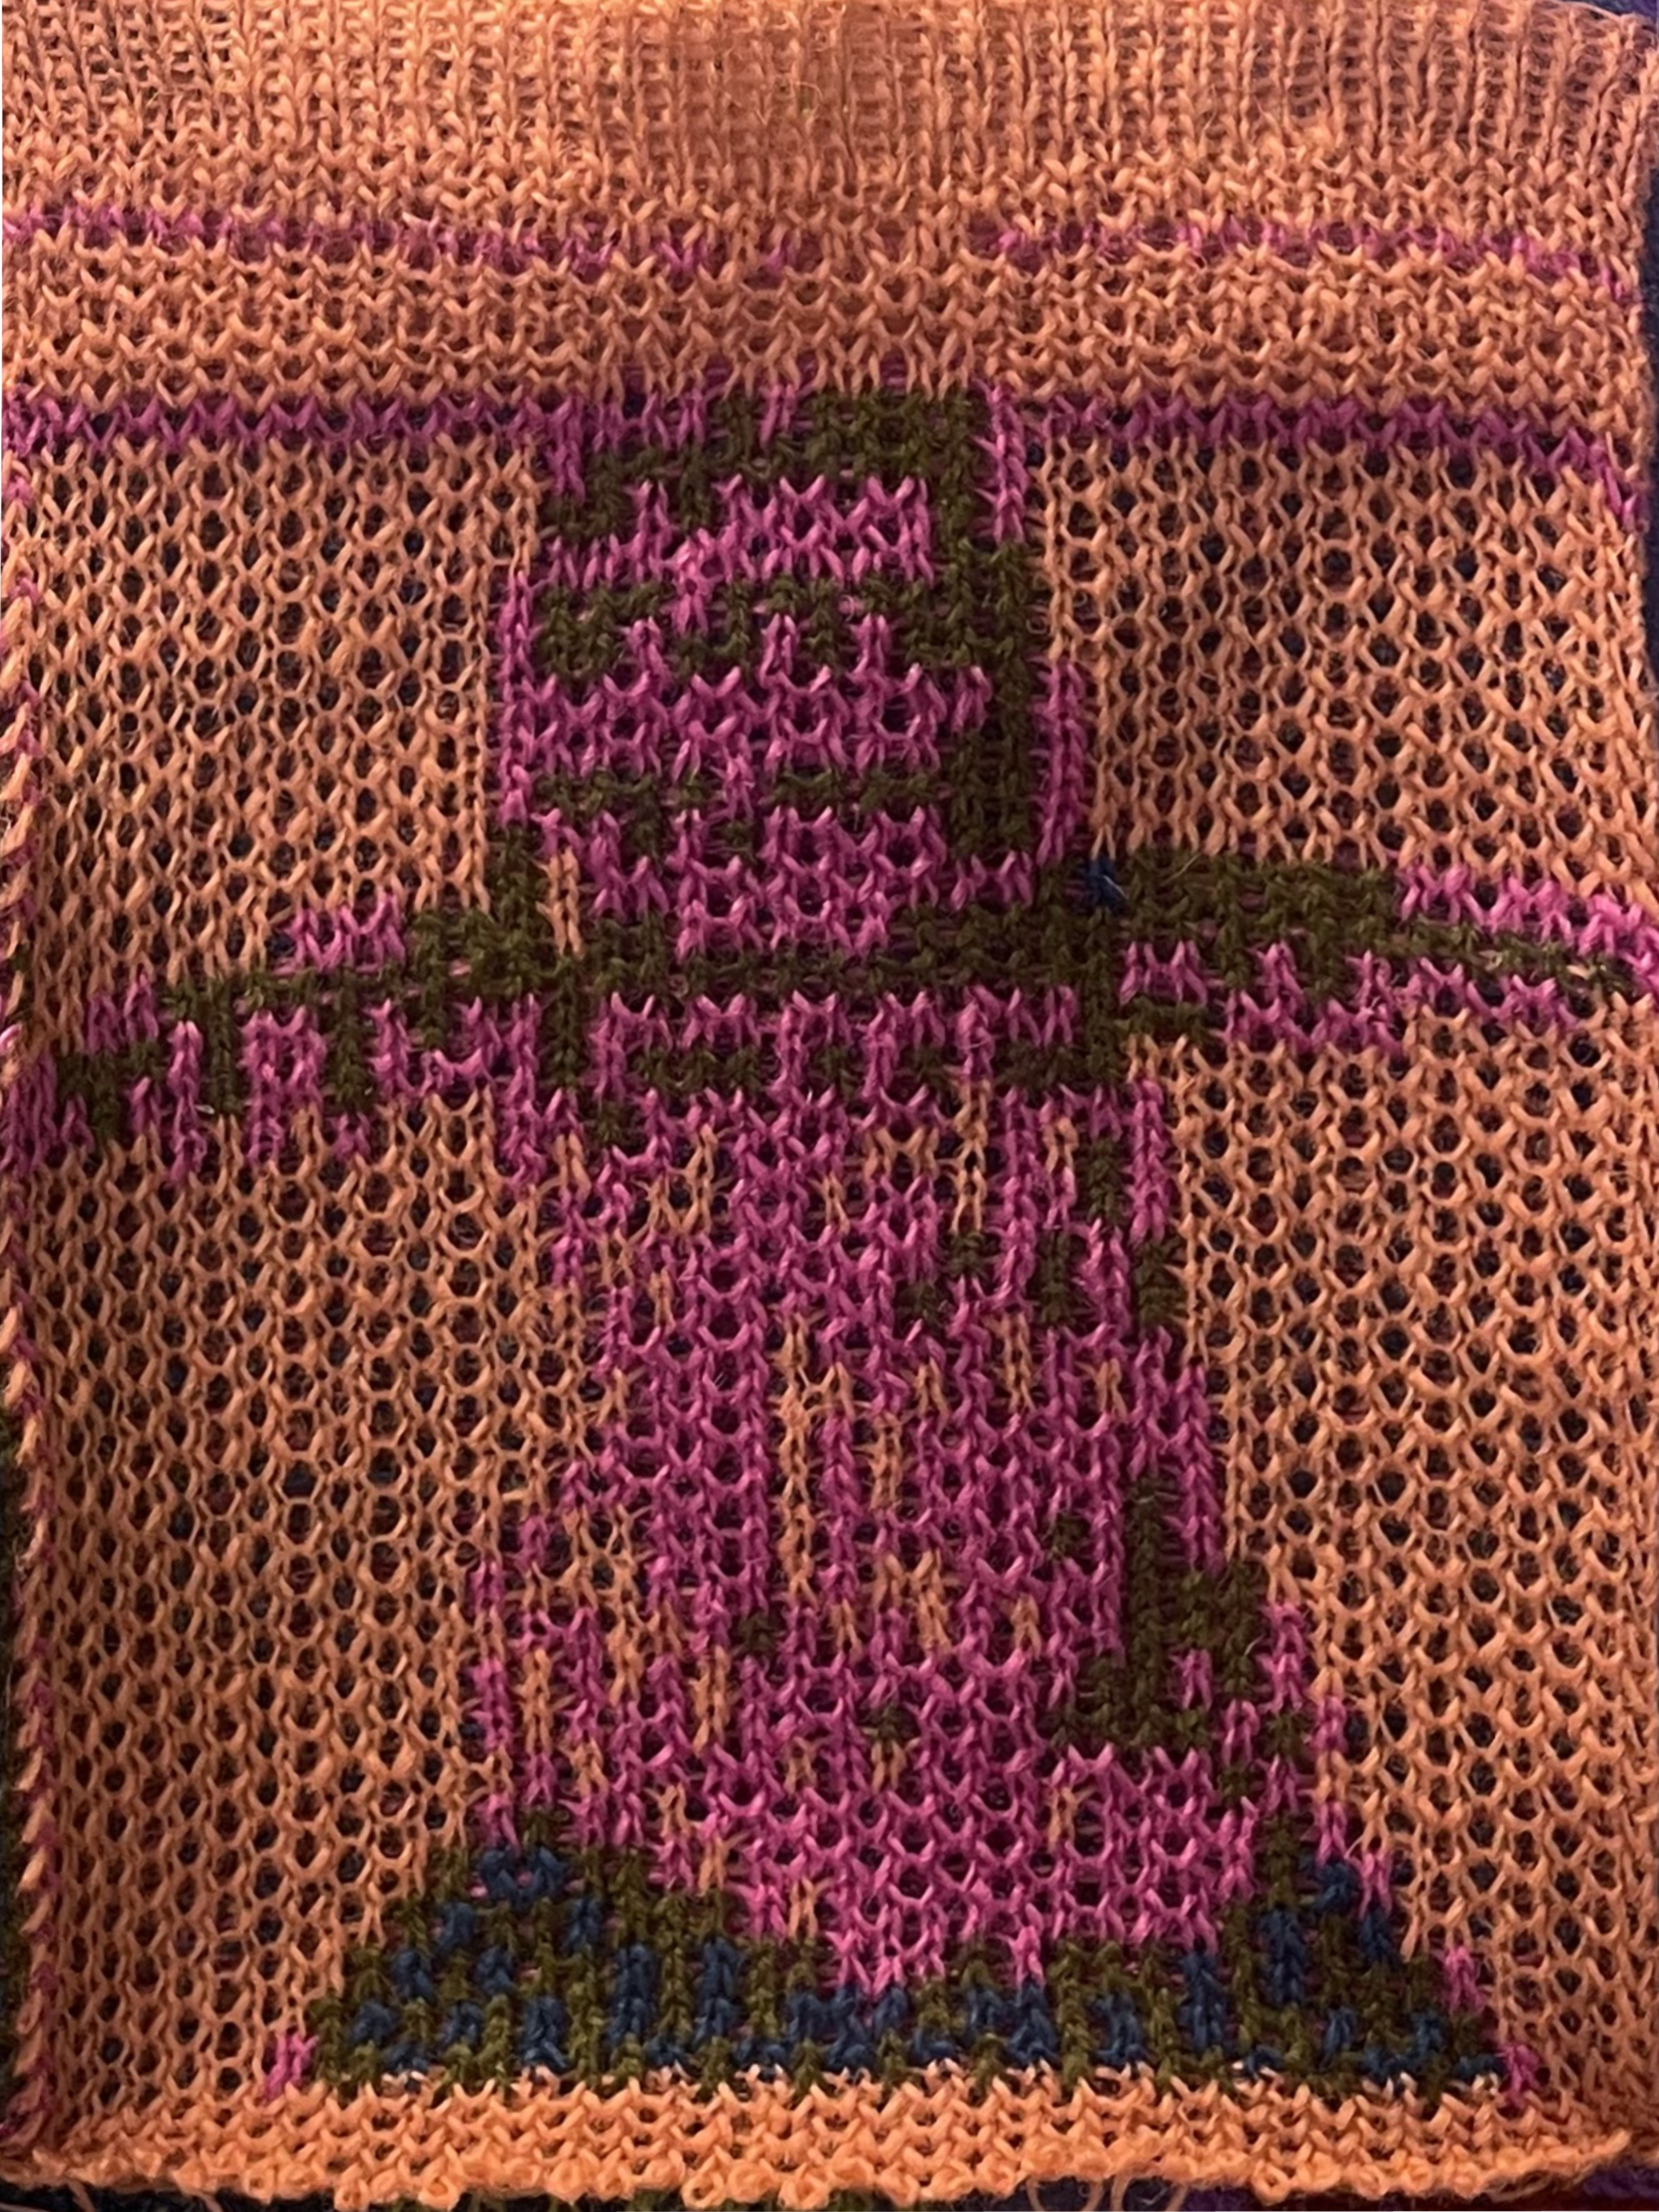
\includegraphics[height=.30\textheight]{myndir/gisa/ragga-lowres.JPG}
    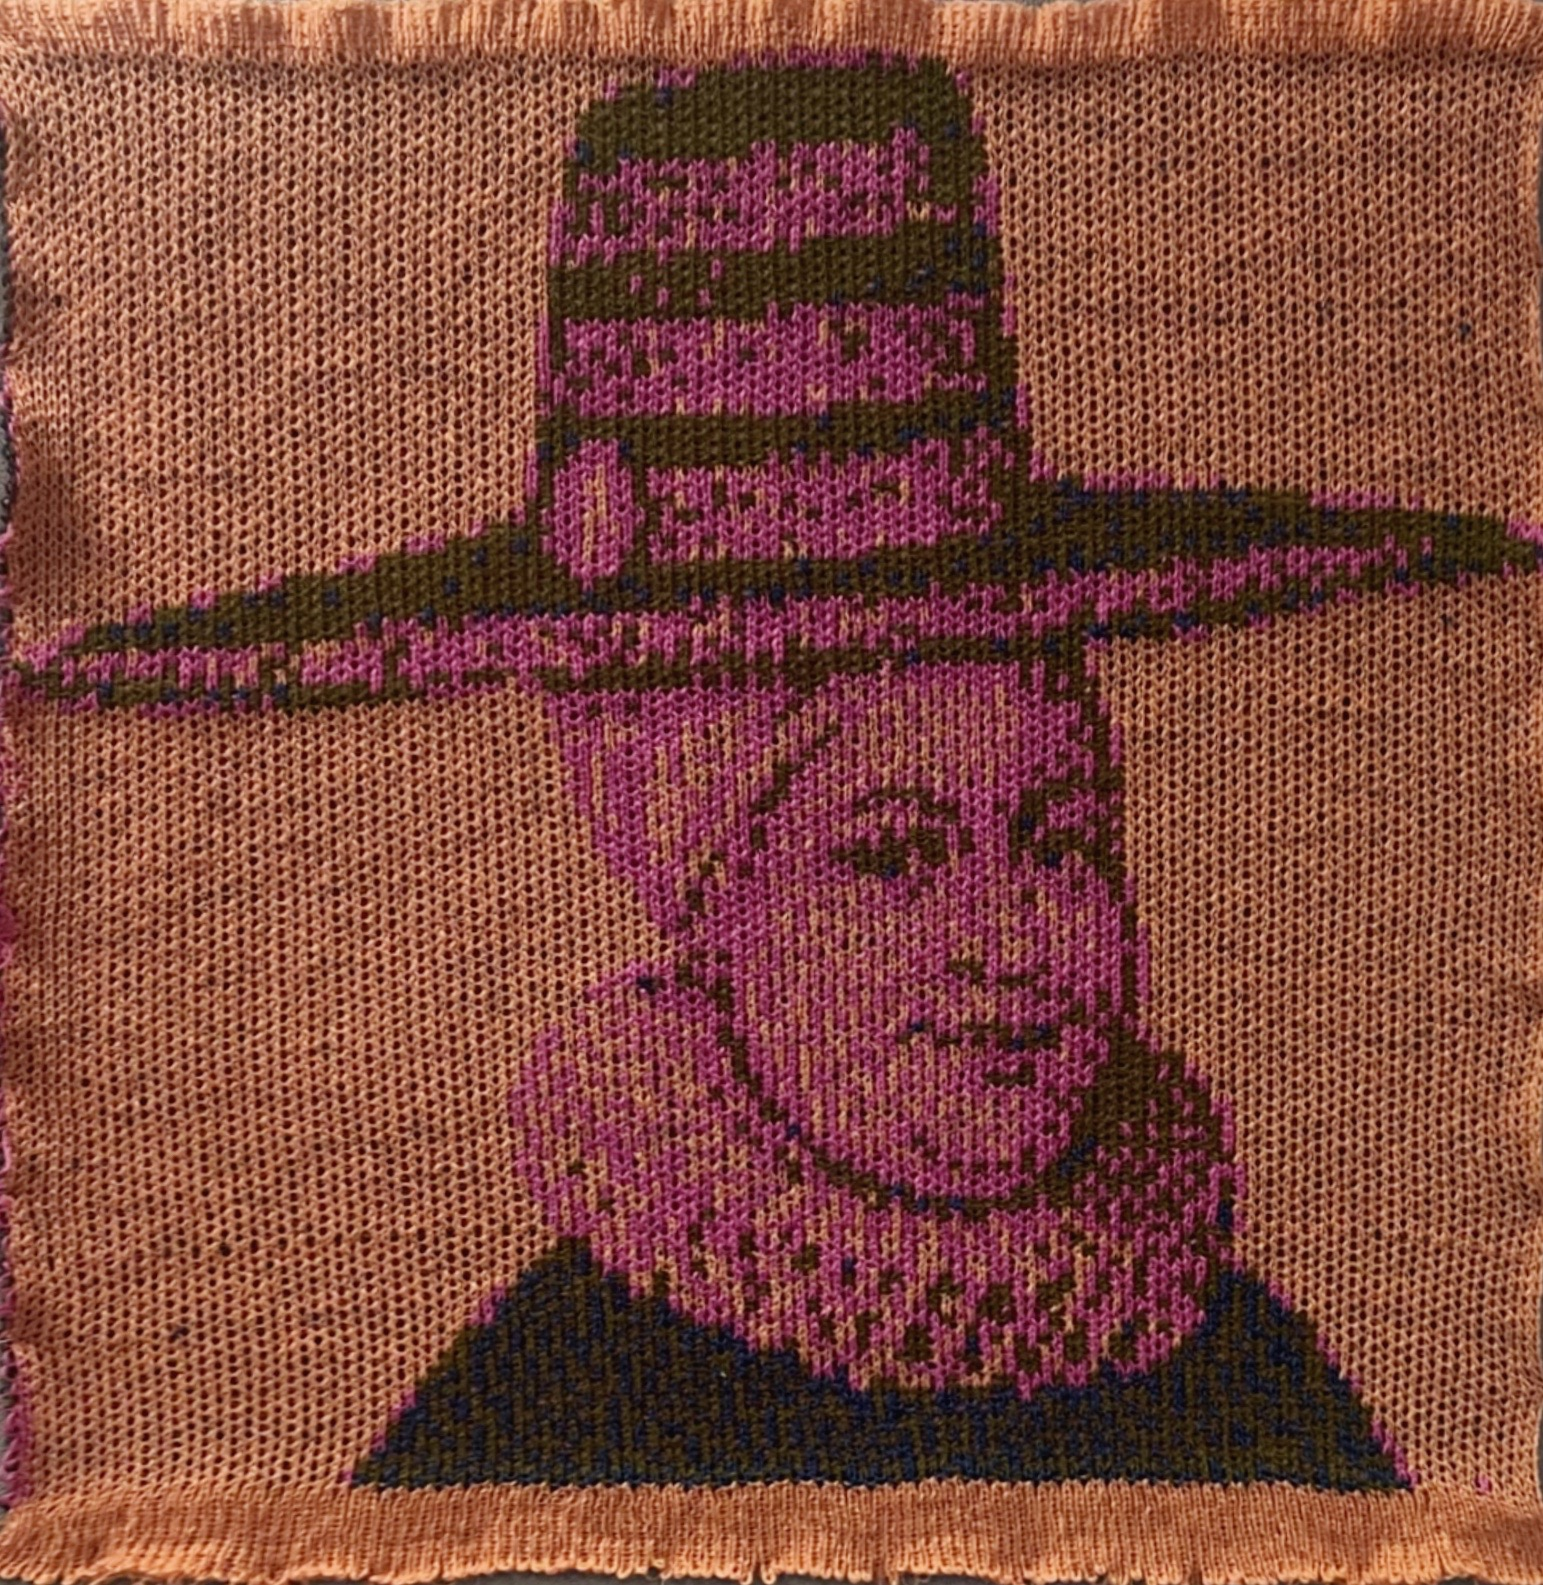
\includegraphics[height=.30\textheight]{myndir/gisa/ragga-hires.JPG}
    \caption{Ragnheiður ,,yngri'' Jónsdóttir: 50 lykkjur á breidd (til vinstri) og 120 lykkjur á breidd (til hægri).}
    \label{fig:ragga:knit}
\end{figure}

\begin{figure}[p]
    \centering
    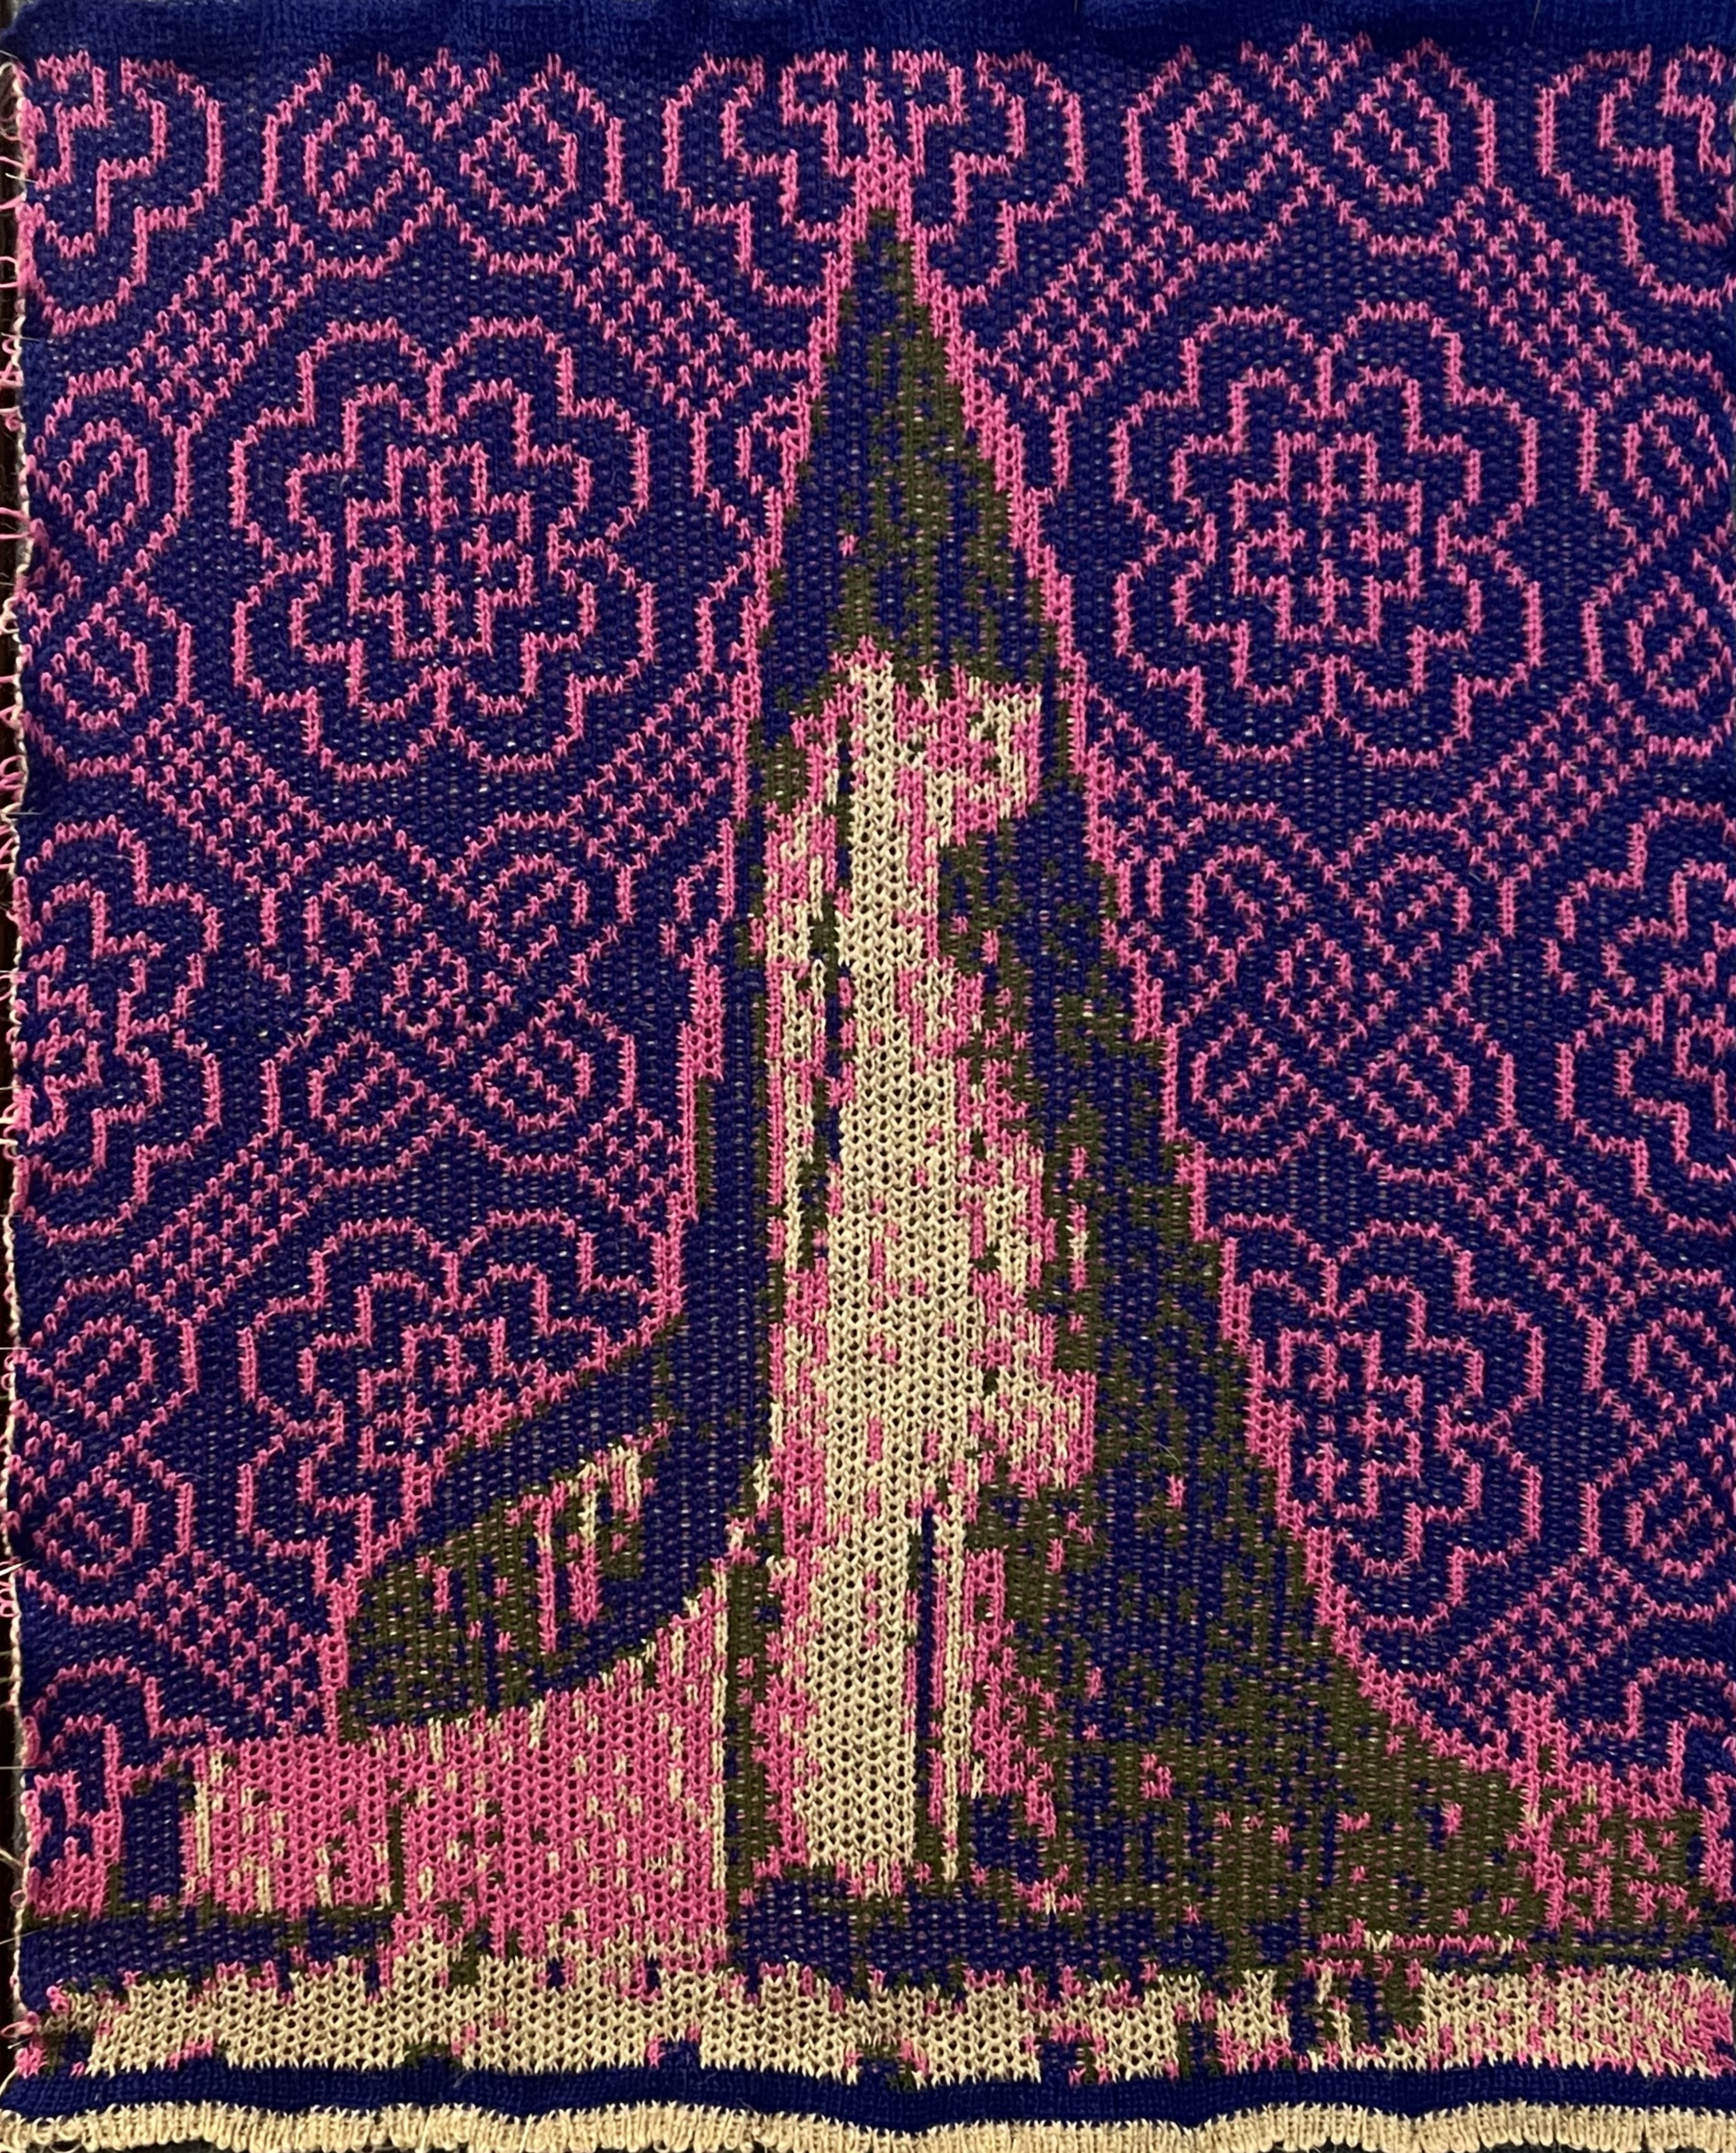
\includegraphics[height=.5\textheight]{myndir/gisa/hallgrimskirkja.JPG}
    \caption{Hallgrímskirkja}
    \label{fig:hallgrimskirkja}
\end{figure}

\newpage
\printbibliography
\fancyfoot{} % clear footer

\begin{center}
\textbf{Nemendur:}
\vspace{2cm}

\underline{\hspace{8cm}} \\
Elías Lúðvíksson \\[1.5cm]

\underline{\hspace{8cm}} \\
Guðrún Ísafold Hilmarsdóttir \\[1.5cm]

\underline{\hspace{8cm}} \\
Snæfríður Ebba Ásgeirsdóttir \\[2cm]

\textbf{Ábyrgðaraðili:} \\[1.5cm]
\underline{\hspace{8cm}} \\
Helga Ingimundardóttir

\end{center}
\end{document}
